% $Author$ $Date$
% http://www.cns.gatech.edu/~predrag/papers/atlas12.pdf

% siminos/atlas/atlas12.tex    pdflatex atlas12
%     then:    pdflatex atlas12; bibtex atlas12; pdflatex atlas12; pdflatex atlas12
% for public version, toggle \draftfalse in setupAtlas.tex
%     (that removes all comments, the blog)

\documentclass[aip,cha,reprint,
secnumarabic,
nofootinbib, tightenlines,
nobibnotes, showkeys, showpacs,
%preprint,%
%reprint,%
%author-year,%
%author-numerical,%
]{revtex4-1}
% aip,cha,preprint,numerical, nofootinbib, groupedaddress

\newcommand{\version}{atlas ver. 0.6, Apr 14 2012}
% Predrag 					ver. 0.6, Apr 14 2012}
% Predrag 					ver. 0.5, Apr 11 2012}
% Predrag 					ver. 0.4, Mar 10 2012}
% Predrag 					ver. 0.3, Mar 10 2012}
% Predrag 					ver. 0.2, Dec 10 2011}
% Predrag 					ver. 0.1, Apr 28 2011}

        \input setupAtlas
        \input ../inputs/def
        \input defAtlas

\begin{document}

\title[High-dimensional cartography]
{Cartography of high-dimensional flows: a visual guide to sections and slices}

%Predrag 2012-04-12: Continuous symmetry reduction of high-dimensional flows
%                    by the method of slices
%Predrag 2012-04-11: How to cut and slice a symmetry
%Predrag 2012-04-11: Have a symmetry? How to cut and slice it
%PC, until 2012-03-19: "Continuous symmetries, and how to slice them"

\author{Predrag Cvitanovi{\'c}}
\email{predrag@gatech.edu.}
\author{Daniel Borrero-Echeverry}
\author{Keith Carroll}
\author{Bryce Robbins}
\author{Lei Zhang}
\affiliation{
 Center for Nonlinear Science and School of Physics,
 Georgia Inst. of Technology,
 Atlanta, GA  30332, USA
}

\date{\today}
%\date{18 December 2011}
%\setcounter{page}{1}

\begin{abstract}
Symmetry reduction by the method of slices quotients the continuous
symmetries of chaotic flows. Within the symmetry reduced state space,
relative equilibria reduce to equilibria, and relative periodic orbits reduce to
periodic orbits. Visualizations of these solutions and their unstable
manifolds reveal their interrelations and the role they play in
organizing turbulence / chaos.

\end{abstract}

\pacs{02.20.-a, 05.45.-a, 05.45.Jn, 47.27.ed, 47.52.+j, 83.60.Wc}
%DB  04/12/2012: Turned PACS on. Use showpacs class option if PACS display desired
%% copied from siminos/blog/strategy.tex
% \PACS 02.20.-a \sep 05.45.-a \sep 05.45.Jn \sep 47.27.ed \sep 47.52.+j
% 02.20.-a      Group theory, mathematics
% 05.45.-a      Nonlinear dynamics and chaos
% 05.45.Jn      High-dimensional chaos
% 47.27.ed      Dynamical systems approaches (turbulent flows)
% 47.52.+j      Chaos in fluid dynamics
% 83.60.Wc      Flow instabilities
% 95.10.Fh      Chaotic dynamics

\keywords{
symmetry reduction,
equivariant dynamics,
relative equilibria,
relative periodic orbits,
slices,
moving frames
}%Use showkeys class option if keyword display desired
\maketitle

\begin{quotation}
Today it is possible to visualize hydrodynamic turbulence as a stroll
through 61,506\dmn\ \statesp. Charting this world is a geometer's task,
and we will map it using a measuring tape, but first one has to deal with
symmetries. Physicists have come to love them inordinately, but Nature
less so: even though the governing equations are symmetric, turbulence
breaks all symmetries, and rather than simplifying our task, for
nonlinear dynamics symmetries obscure the essential dynamics. Evolution
in time decomposes the \statesp\ into spaghetti of time trajectories,
continuous spatial symmetries stratify it into layers of an onion. There
exist many excellent methods that quotient out symmetries of
low-dimensional systems, but so far only one, \mslices, can be mustered
for extremely high-dimensional flows of turbulent fields. In this
geometrical tour of dynamics we show you how to cut this knot and pick a
single point for each trajectory (section it) and each group orbit (slice
it). Once the fog of symmetries is out of the way, one can identify and
describe the prominent fluid structures by taxonomy of its invariant
building blocks: numerically exact solutions of \NSe, finite sets of
\reqva\ and infinite hierarchies of \rpo s, and describe the dynamics in
terms of their heteroclinic connections.
\end{quotation}
%%%%%%%%%%%%%%%%%%%%%%%%%%%%%%%%%%%%%%%%%%%%%%%%%%%%%%%%%%%%%%%%%%%%%%%%%%
%    The first paragraph of the article should be a Lead Paragraph and
%    will be highlighted in the journal in boldface type. This paragraph,
%    which essentially advertises the main points of the article, must
%    describe in terms accessible to the nonspecialist reader the context
%    and significance of the research problem studied and the importance
%    of the results. The Editors will pay special attention to the clarity
%    and accessibility of this paragraph, and in many cases may rewrite it

\section{Introduction}
\label{s:intro}

%%    \DB{2012-04-12}{this is an example how I can alert the co-authors to
%%    a significant edit}

Over the last decade, new insights into the dynamics of moderate
\Reynolds\ turbulent flows have been gained through visualizations of
their $\infty$-dimensional \statesp s by means of dynamically invariant,
representation independent coordinate frames\rf{GHCW07} constructed from
physically prominent unstable {\cohStr s}, hereafter referred to {\em
\template s}.
The most recent advance within this new framework is
the first determination of \rpo s that in part shape turbulence observed
in pipe flows\rf{ACHKW11}. Navigating and charting the geometry of these
extremely high-dimensional \statesp s necessitates a reexamination of two
of the basic tools of the theory of dynamical systems: \PoincSec s and symmetry
reduction\rf{rowley_reconstruction_2000,BeTh04,SiCvi10,FrCv11}. We strive
here to explain the key geometrical ideas in simple but illustrative
settings, eschewing the fluid dynamical and group theoretical
technicalities.

%%%%%%%%%%%%%%%%%%%%%%%%%%%%%%%%%%%%%%%%%%%%%%%%%%%%%%%%%%%%%%%%%%%%%
\begin{figure}
   \centering
  \setlength{\unitlength}{0.20\textwidth}
(a)~~~
  \begin{picture}(1,0.98239821)%
    \put(0,0){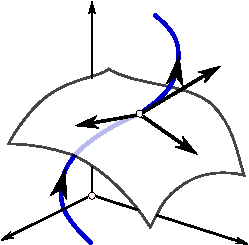
\includegraphics[width=\unitlength]{A28tangent3}}%
    \put(0.91612064,0.70682767){\color[rgb]{0,0,0}\makebox(0,0)[lb]{\smash{$\vel$}}}%
    \put(0.48698745,0.90266503){\color[rgb]{0,0,0}\makebox(0,0)[lb]{\smash{$\ssp(\zeit)$}}}%
    \put(0.2624318,0.5347756){\color[rgb]{0,0,0}\makebox(0,0)[lb]{\smash{$\groupTan_1$}}}%
    \put(0.80471037,0.38188675){\color[rgb]{0,0,0}\makebox(0,0)[lb]{\smash{$\groupTan_2$}}}%
    \put(0.538343,0.25344355){\color[rgb]{0,0,0}\makebox(0,0)[lb]{\smash{$\LieEl\ssp$}}}%
    \put(0.47864531,0.56060893){\color[rgb]{0,0,0}\makebox(0,0)[lb]{\smash{$\ssp$}}}%
  \end{picture}%
~~(b)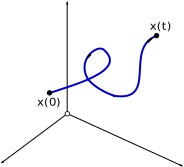
\includegraphics[width=0.20\textwidth]{A27traj}
\\
(c)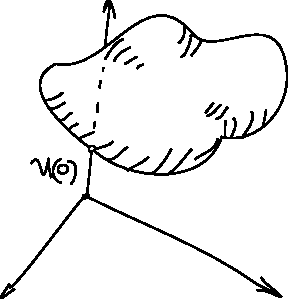
\includegraphics[width=0.20\textwidth]{A27gOrbit}
(d)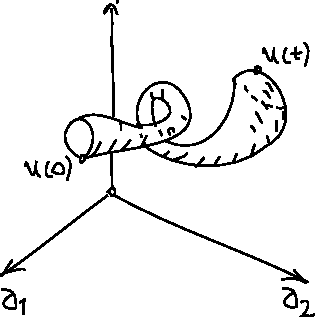
\includegraphics[width=0.20\textwidth]{A27wurst}
   \caption{\label{fig:A27wurst}
   (a)
In presence of $N$-continuous parameter symmetry, each \statesp\ point
$\ssp$ owns $(N\!+\!1)$ tangent vectors: one $\vel(\ssp)$ along the time
flow $\ssp(\zeit)$, and the $N$ group tangents  $\groupTan_1(\ssp), \,
\groupTan_2(\ssp) ,\,\cdots, \groupTan_N(\ssp)$ along infinitesimal
symmetry shifts, tangent to the group orbit $\LieEl\ssp$.
    (b)
Trajectory.
    (c)
Group orbit.
    (d)
Wurst.
}
\end{figure}
%%%%%%%%%%%%%%%%%%%%%%%%%%%%%%%%%%%%%%%%%%%%%%%%%%%%%%%%%%%%%%%%%%%%%

A flow $\map^t$ and the \statesp\ $\pS$ on which the flow acts comprise a
{dynamical system}. If a group $\Group$ of continuous transformations
acts on a continuous time flow, each \statesp\ point owns a set of
tangent vectors (\reffig{fig:A27wurst}\,(a)). Integrated globally, the
velocity vector $\vel(\ssp)$ traces out the {\em trajectory}
$\flow{\zeit}{\ssp}$ ( \reffig{fig:A27wurst}\,(b)). Applying the continuous
transformations traces out the {group orbit} (or, from now on, just
\emph{orbit})
\(
\pS_\ssp = \{\LieEl\,\ssp \mid \LieEl \in {\Group}\}
% \,,\qquad \pS_\ssp \subset \pS
\,
\) %ee{sspOrbit}
(\reffig{fig:A27wurst}\,(c)). Together they trace out a complicated smooth
manifold (hereafter affectionately referred to as the {\em wurst}, see
figures~\ref{fig:A27wurst}\,(d), \ref{fig:CLf01group}\,(b) and
\ref{fig:sliceimage}), that we shall teach you here how to slice.

A flow is said to have symmetry $\Group$ if the form of evolution
equations $\dot{\ssp} = \vel(\ssp)$ is left invariant,
\(
\vel(\ssp)=\LieEl^{-1} \, \vel(\LieEl \, \ssp)
% \,,\qquad \mbox{for all }
\,,
\) %ee{eq:FiniteRot}
by the set of transformations $\LieEl \in {\Group}$. Physicists love
symmetry, but Nature does not care: turbulence breaks all symmetries,
and while the flow equations may be invariant under $\Group$, their
solutions typically are not.

The key to chaotic dynamics is the notion of recurrence. To quantify how
close the state of the system now is to a previously visited state, we
need the notion of distance between two points in \statesp. The simplest
(but far from the only, or the most natural) is the Euclidean norm
\beq
  \Norm{\ssp-\ssp'}^2  = \braket{\ssp-\ssp'}{\ssp-\ssp'} =
\sum_j^d
(\ssp-\ssp')_j^2
\,.
\ee{innerproduct}
Given a notion of distance we can talk about 'neighborhood,' the open set of
nearby states. Our main task in what follows will be to make this precise,
by defining a chart over a neighborhood, and its borders.
Given distances and neighborhoods,
the next key notion is  \emph{measure}, or how likely a typical
trajectory is to visit a given neighborhood. After some observations of a
given turbulent flow, one can identify a set of representative
\emph{\template s}\rf{rowley_reconstruction_2000}, {points}
$\slicep{}^{(j)}$, $j=1,2,\cdots$ in the \statesp\ $\pS$, which are the
dynamically most important unstable {\recurrStr s} of the flow.

Our goals here are two-fold:
(i) In \refsect{s:cut} we review the method of \PoincSec s, with
    emphasis on aspects applicable to high-dimensional flows: construction of
    multiple local linear `charts' and determination of their borders and
(ii) in \refsect{s:slice} we show how the same set of tools applied to
    reduction of continuous symmetries enables us to commence a
    systematic charting of the long-time dynamics of high-dimensional
    flows with continuous symmetries (\refsect{s:chart}).


\section{Section}
\label{s:cut}

In the {\em \PoincSec} method one records the coordinates
$\sspRed_n$ of the trajectory $\ssp(\zeit)$ at the instants $\zeit_n$
when it traverses a fixed oriented hypersurface $\PoincS$ of codimension
1. For high-dimensional flows that we have in mind, the practical choice
is a hyperplane, the only type of \PoincSec\ (from now on, just a
\emph{section}) we shall consider here. Such a section captures
important features of the flow in an open neighborhood of the
section-fixing \template.

As an example consider the system of R\"ossler\rf{ross},
\index{R\"ossler system}
\beq
\begin{split}
  \dot{x} &= -y \,-\,z \\
  \dot{y} &= x + a y \\
  \dot{z} &= b + z (x - c)
  \,,
  \label{eq:Rossler}
\end{split}
\eeq
where $a = b = 0.2$ and $c = 5.7$. This flow has two prominent invariant
states, the `inner' and the `outer' unstable \eqva\ $\slicep{}^{(-)}$  and
$\slicep{}^{(+)}$, which we pick as {\em \template s} (\refFig{fig:RoessTrjs}).

We orient the sections so the plane $\PoincS_{-}$ contains the 1\dmn\
stable eigenvector of $\slicep{}^{(-)}$ (\reffig{fig:RoessTrjs}\,(b)),
and the other section $\PoincS_{+}$ contains the 1\dmn\ unstable
eigenvector of $\slicep{}^{(+)}$ (\reffig{fig:RoessFarEq}\,(a)), thus
capturing the local spiral-in, spiral-out dynamics. The remaining freedom
to rotate each section can be used to orient them in such a way that the
ridge (the intersection of the two sections) lies approximately
between the two templates (\reffig{fig:RoessFarEq}\,(b)).

A well chosen section captures the dynamics in the neighborhood of its
\template, but how far does this neighborhood extend?
The answer is that the section captures neighboring trajectories as long
as it cuts them transversally; it fails the moment the velocity field at
a point $\sspRSing$ fails to pierce the section. At these locations, the
velocity either vanishes (\eqv) or is tangent to the section, \ie,
orthogonal to the section normal $\hat{n}$,
\beq
    \hat{n} \cdot \vel(\sspRSing) = 0
\,,\qquad
    \sspRSing \in \cal{S}
\,.
\ee{eq:sspRSing}
For a smooth flow such points form a smooth $(d\!-\!2)$\dmn\
\emph{\poincBord} ${\cal S} \subset \PoincS$, which encloses the open
neighborhood of the {\template} characterized by qualitatively similar
flow. We shall refer to this region of the section as a `chart' of the
{\template} neighborhood (see
\reffig{fig:RoessTrjs}\,(b) and \reffig{fig:RoessFarEq}). Beyond the border, the flow
pierces the section hyperplane in the `wrong' direction and the dynamics
are qualitatively different.

%%%%%%%%%%%%%%%%%%%%%%%%%%%%%%%%%%%%%%%%%%%%%%%%%%%%%%%%%%%%%%%%%%%%%
\begin{figure}
(a)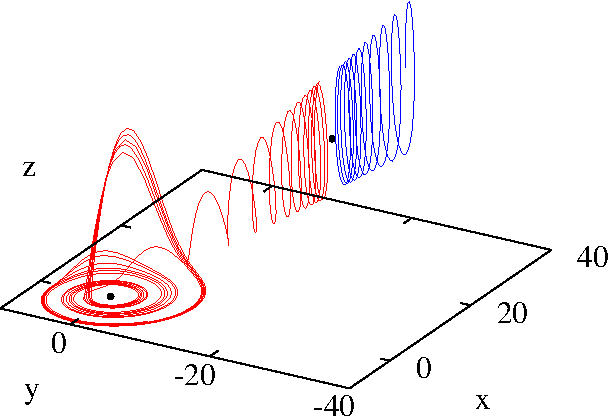
\includegraphics[width=0.24\textwidth]{Rossler_Equilibria}%{RoessTrjs}%
(b)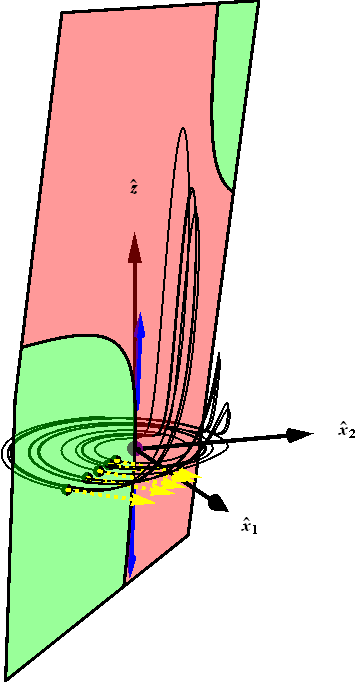
\includegraphics[width=0.18\textwidth,clip=true]{RoessNearEq2a}
    \caption{
(a)
\mycomment{\DBedit{\Huge [DRAW THIS!]}}{}
R\"ossler \eqva\ and their invariant manifolds. The stable manifold of
the inner {\eqv} $\slicep{}^{(-)}$  is 1-dimensional and the unstable one
is a spiral-out focus. For the outer {\eqv} $\slicep{}^{(+)}$  the stable
manifold is a spiral-in focus (basin boundary for initial conditions that
either fall into the chaotic attractor, or escape to infinity) and the
unstable manifold is 1-dimensional.
(b)
\PoincSec\ plane through the inner {\eqv} $\slicep{}^{(-)}$ and
its stable eigenvector. The chart $\PoincS_{-}$ of the $\slicep{}^{(-)}$
neighborhood, bounded by its \poincBord, is highlighted by (light) green.
    }
\label{fig:RoessTrjs}
\end{figure}
%%%%%%%%%%%%%%%%%%%%%%%%%%%%%%%%%%%%%%%%%%%%%%%%%%%%%%%%%%%%%%%%%%%%%

%%%%%%%%%%%%%%%%%%%%%%%%%%%%%%%%%%%%%%%%%%%%%%%%%%%%%%%%%%%%%%%%%%%%%
% supercedes \label{fig:RoessBothEq}
\begin{figure}%[H]
\begin{center}
(a)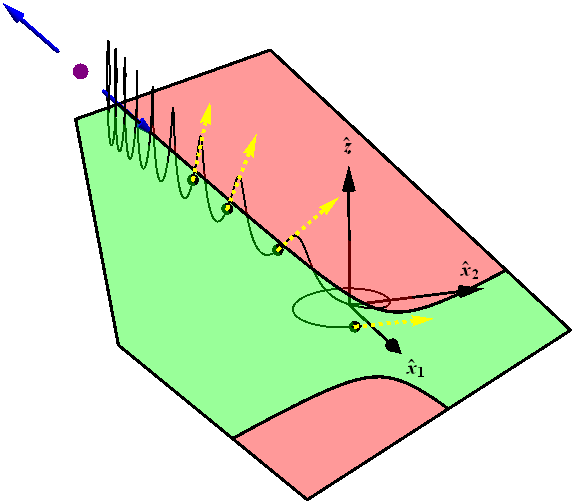
\includegraphics[width=0.23\textwidth,clip=true]{RoessFarEq2}%
(b)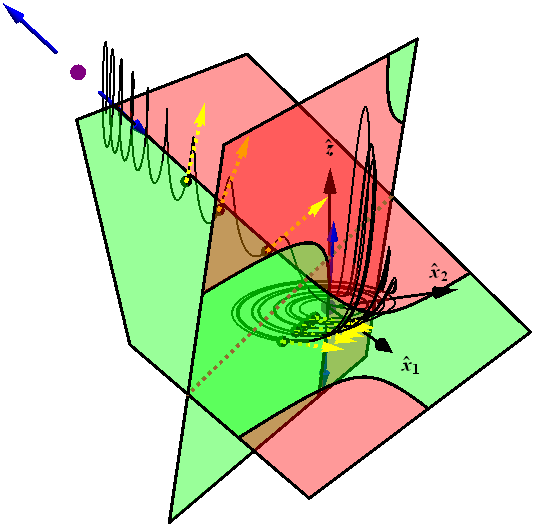
\includegraphics[width=0.23\textwidth,clip=true]{RoessSctAtlas2}
\end{center}
  \caption[R\"ossler section, outer {\eqv}]{
(a)
  A section through the outer {\eqv} $\slicep{}^{(+)}$  and its unstable
  eigenvector. The velocity $\vel(\sspRed_n)$ at the $n$th section is
  indicated by (yellow) vector.
(b)
  A two-chart atlas of R\"ossler flow, with charts $\PoincS_{-}$ and
  $\PoincS_{+}$ oriented and combined so that the ridge (intersection of
  the two sections, indicated by the dotted brown line) lies
  approximately between the \template s.
  } \label{fig:RoessFarEq}
\end{figure}
%%%%%%%%%%%%%%%%%%%%%%%%%%%%%%%%%%%%%%%%%%%%%%%%%%%%%%%%%%%%%%%%%%%%%

For R\"ossler flow, the border condition \refeq{eq:sspRSing} yields a
quadratic condition in 3 dimensions, so \poincBord s\ drawn in
\reffig{fig:RoessTrjs}\,(b) and \reffig{fig:RoessFarEq} are conic
sections. The two charts meet at a ridge, and together do a pretty good
job as the 2-chart atlas of the interesting R\"ossler dynamics,
\reffig{fig:RoessFarEq}. As explained in ChaosBook.org\cite{DasBuch}, due
to extreme contraction rate, the section in \reffig{fig:RoessTrjs}\,(b)
is for all practical purposes 1\dmn, and the associated return map yields
all \po s of the 3\dmn\ flow.

In 3 dimensions everything -sections, ridges, \poincBord s- can be
drawn, and a $\chi\alpha\rho\tau\eta\varsigma$ does fit on a sheet of
papyrus. But what about high-dimensional flows? The point of the
cartography enterprize undertaken here is that while it is impossible to
visualize  61,504% 61,506-2 $(d\!-\!2)$
\dmn\ {\poincBord} of the 61,505% 61,506-1 $(d\!-\!1)$
\dmn\ slab that is now our chart\rf{GibsonMovies}, a point is a point,
and a line is a line in a projection from any number of dimensions, so a
trajectory crossing of both a section and a {\poincBord} can be easily
determined and visualized in any dimension.

To summarize:
Evolution in time decomposes the \statesp\ into a spaghetti of 1\dmn\
trajectories $\ssp(\zeit)$, each determined by a single point $\ssp(0)$
on it. A well chosen set of \emph{sections} of codimension 1 allows us to
`quotient' the continuous time parameter $\zeit$. For unstable
trajectories one needs, in addition, a notion of recurrence to the
section. The set of points $\{\sspRed_n\} = \{\ssp(\zeit_n)\}$,  separated
by short-time section to section flights, then captures the transverse
dynamics without losing any information about the chaotic flow.
We can thus chart the regions of \statesp\ of interest, by a picking a
sufficient number of \template s and the associated charts over their
neighborhoods, each bounded by \poincBord s and ridges.

Two concluding remarks on what sections \emph{are not}:

(1) A \PoincSec\ is {\em not} a projection onto a
lower-dimensional space: Rather, it is a local change of coordinates to a
direction along the flow $\vel(\sspRed)$, and the remaining coordinates
transverse to it. No information about the flow is lost; the full space
trajectory can always be reconstructed by integration from its point
$\sspRed$ in the section.

(2) The method of \PoincSec s is {\em not} equivalent to
\emph{strobing} a flow at a sequence of instants in time. While
`strobing' is what any numerical integrator does, by representing a
trajectory by a sequence of time-integration step separated points, this
is no reduction of a flow to a codimension 1 manifold, as the sequence of
strobed points still resides in the full \statesp\ $\pS$, of
dimensionality $d$.


\section{Dancers and drifters}
% and symmetries}
% Dynamics and symmetry
\label{s:symm}

%% A27*-pipeSymms.* - read dasbuch/book/FigSrc/inkscape/00ReadMe.txt
 \begin{figure}
 \begin{center}
  \setlength{\unitlength}{0.20\textwidth}
  %% \unitlength = units used in the Picture Environment
(a)
  \begin{picture}(1,0.52454249)%
    \put(0,0){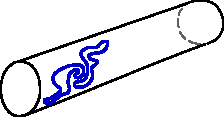
\includegraphics[width=\unitlength]{A27a-pipeSymms}}%
    \put(0.61583231,0.13683004){\color[rgb]{0,0,0}\makebox(0,0)[lb]{\smash{$z$}}}%
    \put(0.00611823,0.27217453){\color[rgb]{0,0,0}\makebox(0,0)[lb]{\smash{$\theta$}}}%
  \end{picture}%
(b)
  \begin{picture}(1,0.52454249)%
    \put(0,0){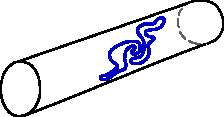
\includegraphics[width=\unitlength]{A27b-pipeSymms}}%
    \put(0.61583231,0.13683004){\color[rgb]{0,0,0}\makebox(0,0)[lb]{\smash{$z$}}}%
    \put(0.00611823,0.27217453){\color[rgb]{0,0,0}\makebox(0,0)[lb]{\smash{$\theta$}}}%
  \end{picture}%
\\
(c)
  \begin{picture}(1,0.52454249)%
    \put(0,0){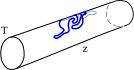
\includegraphics[width=\unitlength]{A27c-pipeSymms}}%
    \put(0.61583231,0.13683004){\color[rgb]{0,0,0}\makebox(0,0)[lb]{\smash{$z$}}}%
    \put(0.00611823,0.27217453){\color[rgb]{0,0,0}\makebox(0,0)[lb]{\smash{$\theta$}}}%
  \end{picture}%
(d)
  \begin{picture}(1,0.52454249)%
    \put(0,0){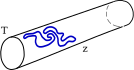
\includegraphics[width=\unitlength]{A27d-pipeSymms}}%
    \put(0.61583231,0.13683004){\color[rgb]{0,0,0}\makebox(0,0)[lb]{\smash{$z$}}}%
    \put(0.00611823,0.27217453){\color[rgb]{0,0,0}\makebox(0,0)[lb]{\smash{$\theta$}}}%
  \end{picture}%
 \end{center}
 \caption[$\On{2}_\theta \times \SOn{2}_z$ symmetry of flow in a stream-wise
          periodic pipe]{
A fluid state in a pipe translated or rotated is
also a solution. In particular, a \rpo\ $\pS_p$ is
(a) a \emph{time dependent} state of the fluid that after a period $\period{p}$ reemerges
(b) translated by downstream shift $\shift_p$
(such solutions are stream-wise periodic pipe $\SOn{2}_z$ equivariant),
(c) translated by downstream shift $\shift_p$ and rotated azimuthally by $\gSpace_p$
(i.e., $\SOn{2}_{\phi} \times \SOn{2}_z$ equivariant) or,
(d) reflected and rotated azimuthally by $\gSpace$ (i.e., $\On{2}_{\phi}$ equivariant).
Consider this in contrast to a \reqv, a constant shape that travels
downstream with constant {\phaseVel} $\velRel$. (from \wwwcb{})
 }\label{fig:A27-pipeSymms}
 \end{figure}
%% A27*-pipeSymms.* %%%%%%%%%%%%%%%%%%%%%%%%%%%%%%%%%%%%%%%%%%%%%%%%%%%%%%%

What is a symmetry? A visualization of the fluid dynamics of a pipe flow,
\reffig{fig:A27-pipeSymms}, affords an intuitive illustration. Solutions
of pipe flow remain physically the same under azimuthal rotations and
stream-wise translations (which become \SOn{2} rotations in numerical
stream-wise periodic pipes) but correspond to different points in
\statesp\ and may look very different in its visualizations.

Each \SOn{2} group orbit is topologically a circle, but it traces out a
complicated \statesp\ curve composed of many Fourier modes nonlinearly
coupled and thus of comparable magnitudes. Together
the two \SOn{2} sweep out contorted and hard to visualize $T^2$ tori (see
\refref{ACHKW11}), but we shall illustrate here the key ideas by a much
simpler example, the $\SOn{2}$-equivariant Gibbon and
McGuinness\rf{GibMcCLE82,FowlerCLE82} \cLe\ of geophysics and laser
physics,
\bea
	\dot{x}_1 &=& -\sigma x_1 + \sigma y_1
        \,,\qquad
	\dot{x}_2 \,=\, -\sigma x_2 + \sigma y_2
        \continue
	\dot{y}_1 &=& (\RerCLor-z) x_1 - \ImrCLor x_2 -y_1-e y_2 \continue
	\dot{y}_2 &=& \ImrCLor x_1 + (\RerCLor-z) x_2 + e y_1- y_2\continue
	\dot{z} \; &=& -b z + x_1 y_1 + x_2 y_2
    \,.
\label{eq:CLeR}
\eea
Here the parameters are set to Siminos's values $\RerCLor=28,\,
\ImrCLor=0,\, b=8/3,\, \sigma=10,\, e= 1/10$. (For the background and an
in-depth investigation of the model  see \refrefs{SiminosThesis,SiCvi10}.)

\begin{figure}
  	\begin{center}
  	\setlength{\unitlength}{0.20\textwidth}
  (a)
  	\begin{picture}(1,1.07802818)%
    	\put(0,0){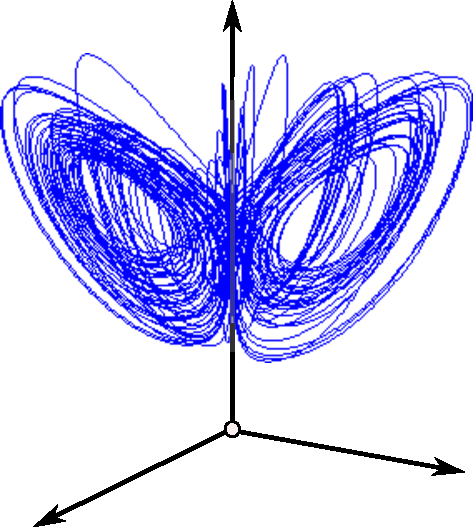
\includegraphics[width=\unitlength]{CLEattractor}}%
    	\put(0.55152995,1.0139628){\color[rgb]{0,0,0}\makebox(0,0)[lb]{\smash{$z$}}}%
    	\put(0.05573445,0.0739776){\color[rgb]{0,0,0}\makebox(0,0)[lb]{\smash{$x_1$}}}%
    	\put(0.90013492,0.16491708){\color[rgb]{0,0,0}\makebox(0,0)[lb]{\smash{$x_2$}}}%
  	\end{picture}%	
  (b)
  	\begin{picture}(1,1.06440474)%
    	\put(0,0){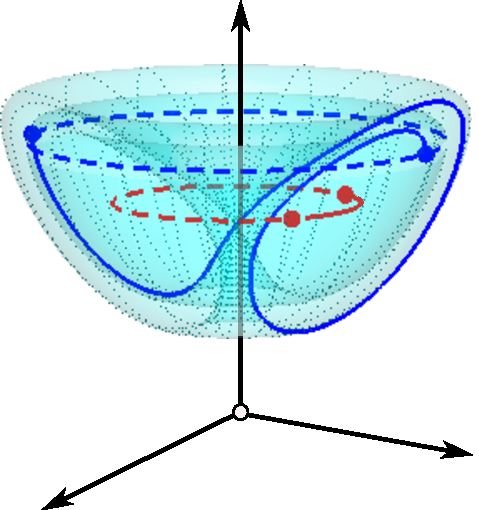
\includegraphics[width=\unitlength]{CLEWurst01}}%
   		\put(0.55961552,1.00214901){\color[rgb]{0,0,0}\makebox(0,0)[lb]{\smash{$z$}}}%
   		\put(0.07008555,0.07304272){\color[rgb]{0,0,0}\makebox(0,0)[lb]{\smash{$x_1$}}}%
    	\put(0.90381504,0.16283301){\color[rgb]{0,0,0}\makebox(0,0)[lb]{\smash{$x_2$}}}%
  	\end{picture}	
    \end{center}
  \caption
  [\CLf: $\cycle{01}$ {\rpo} group orbit]{
  (a)
  The strange attractor of \cLf.
  (b)
  The initial \reqv\ $\REQV{}{1}$ point is shown by the red dot, and its
  group orbit / trajectory by the dashed red line. One period of the
  $\cycle{01}$ {\rpo} is shown by the solid blue line. The group orbit of
  its (arbitrary) starting point is shown by the dashed blue line: after
  one period the trajectory has returned to the group orbit but with a
  different phase. The wurst, \ie, the group orbit of the $\cycle{01}$
  trajectory (dark blue) is shown by the cyan surface. Trajectory of the
  further 15 repeats of $\cycle{01}$ (faint dotted lines) traces out this
  torus; in that time the slowly drifting \reqv\ $\REQV{}{1}$ has
  advanced to the next red dot (red line).
  }
\label{fig:CLf01group}
\end{figure}

The strange attractor of the \cLf\ is shown in
\reffig{fig:CLf01group}\,(a). It is a mess. Why? The problem of dynamics
in presence of symmetry can perhaps be understood this way: dissipative
flows settle into solutions with low friction. Since drifting along the
non-shape-changing symmetry directions is energetically cheap, rather
than do work, solutions tend to drift along. Thus, the physically
important shape-changing dynamics are smeared out.
%DB 4/13/2012: I think this is the general idea, but not sure how much of a claim this is
    \KC{2012-04-13}{I do not understand the paragraph. Predrag: did
                    Daniel's edit help?}

A continuous symmetry leads to drifting invariant solutions. A {\em
\reqv} (traveling wave, rotational wave, ...) is a trajectory whose
velocity field lies within the group tangent space, such that
\(
\vel(\ssp) = c \cdot \groupTan(\ssp)
\) %\label{phaseVel}
with a constant {\phaseVel} $c$, and whose time evolution is thus
confined to the group orbit; think of an unchanging body carried by a
stream.

A {\em \rpo} $\pS_p$ is a trajectory which exactly recurs
\beq
\ssp(\zeit) = \LieEl_p \, \ssp(\zeit + \period{p} )
    \,,\qquad
\ssp(\zeit) \in \pS_p
\ee{RPOrelper1}
after a fixed {relative period} $\period{p}$, but shifted by a fixed
group action ${\LieEl}$ that maps the endpoint $\ssp (\period{p}) $ back
into the initial point cycle point $\ssp (0) $; think of a dancer moving
across the stage through a set of motions and then striking the initial
pose\rf{ShWi06}, or study the pipe flow sketches \reffig{fig:A27-pipeSymms}.

As the $\SOn{2}$ transformations act on the \cLf\ only through the
simplest, $m=1$ Fourier mode, here all group orbits are circles, and appear
elliptical in most $d=5 \to 3$~dimensions projections. Nevertheless, even
the wurst traced out by the very simplest, short \rpo\ $\cycle{01}$ shown
in \reffig{fig:CLf01group}\,(b) is not so easy to get one's head around:
you are looking at a 3\dmn\ projection of a \emph{torus} embedded in 5
dimensions.

%%%%%%%%%%%%%%%%%%%%%%%%%%%%%%%%%%%%%%%%%%%%%%%%%
% 2011-09-09, 2012-03-30 Predrag: add BeThMovFr to
%            continuous.tex overheads, and ChaosBook
% replace A27movFrame*.* everywhere
\begin{figure}
 \begin{center}
  \setlength{\unitlength}{0.20\textwidth}
  %% \unitlength = units used in the Picture Environment
(a)~~
  \begin{picture}(1,0.98655417)%
    \put(0,0){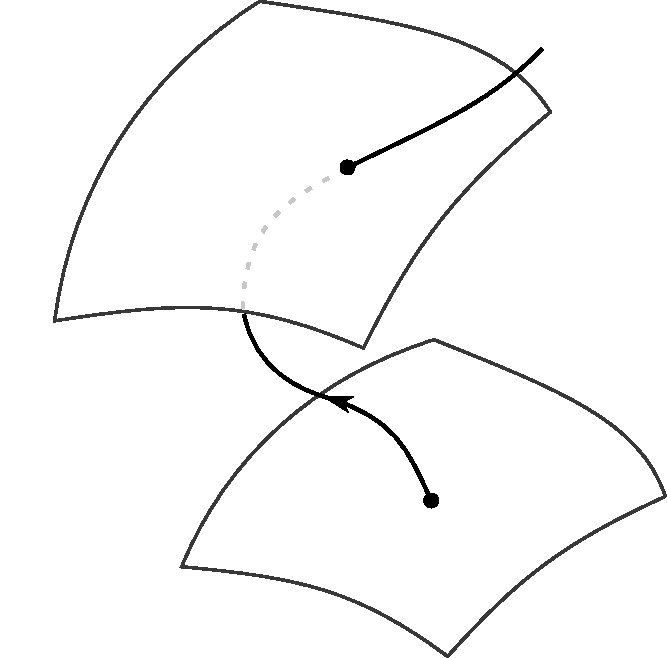
\includegraphics[width=\unitlength]{BeThTrajTeX}}%
    \put(0.35976094,0.91875614){\color[rgb]{0,0,0}\rotatebox{-31.32889204}{\makebox(0,0)[lb]{\smash{$\pS_{\ssp(\zeit)}$}}}}%
        \put(0.60333631,0.42274457){\color[rgb]{0,0,0}\rotatebox{-40.8073288}{\makebox(0,0)[lb]{\smash{$\pS_{\ssp(0)}$}}}}%
    \put(0.66001383,0.16959019){\color[rgb]{0,0,0}\rotatebox{0.0313674}{\makebox(0,0)[lb]{\smash{$\ssp(0)$}}}}%
    \put(0.5058276,0.64524238){\color[rgb]{0,0,0}\rotatebox{0.0313674}{\makebox(0,0)[lb]{\smash{$\ssp(\zeit)$}}}}%
    \put(0.13110825,0.05766516){\color[rgb]{0,0,0}\rotatebox{0.11031334}{\makebox(0,0)[lb]{\smash{$\pS$}}}}%
  \end{picture}%
~~(b)
  \begin{picture}(1,0.98655417)%
    \put(0,0){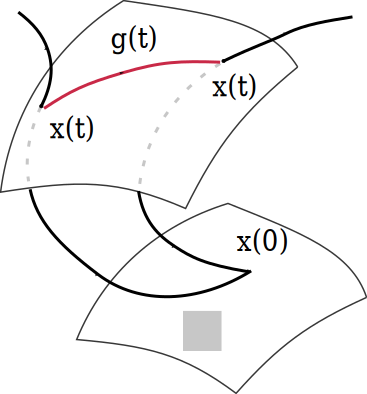
\includegraphics[width=\unitlength]{BeThMovFr}}%
    \put(0.20559239,0.64023845){\color[rgb]{0,0,0}\rotatebox{0.0313674}{\makebox(0,0)[lb]{\smash{$\ssp(\zeit)$}}}}%
    \put(0.67382401,0.35781161){\color[rgb]{0,0,0}\rotatebox{0.0313674}{\makebox(0,0)[lb]{\smash{$\ssp(0)$}}}}%
    \put(0.61221026,0.74589514){\color[rgb]{0,0,0}\rotatebox{0.0313674}{\makebox(0,0)[lb]{\smash{$\sspRed(\zeit)$}}}}%
    \put(0.35760559,0.8662057){\color[rgb]{0,0,0}\rotatebox{0.0313674}{\makebox(0,0)[lb]{\smash{$\LieEl(\zeit)$}}}}%
  \end{picture}%
 \end{center}
  \caption{\label{fig:BeThMovFr}
(a)
The group orbit $\pS_{\ssp(0)}$ of \statesp\ point $\ssp(0)$, and the
group orbit $\pS_{\ssp(\zeit)}$ reached by the trajectory $\ssp(\zeit)$ a time $\zeit$
later.
(b)
The two physically equivalent flows
$\ssp(\zeit)=\LieEl(\zeit)\,\sspRed(\zeit)$ are related by, in general,
an arbitrary, time dependent {\em moving frame} transformation
$\LieEl(\zeit)$.
(from \wwwcb{}).
  }
\end{figure}
%%%%%%%%%%%%%%%%%%%%%%%%%%%%%%%%%%%%%%%%%%%%%%%%%%

To summarize: continuous symmetries of dynamics stratify the \statesp\
into an onion, each layer a group orbit (\reffig{fig:BeThMovFr}). We are
free to replace a given flow $\ssp(\zeit)$ by another, physically
equivalent flow $\ssp(\zeit)=\LieEl(\zeit)\,\sspRed(\zeit)$ by any, in
general, time dependent {\em moving frame} transformation
$\LieEl(\zeit)$. For example, to film our dancer we can mount the camera
on a cart moving alongside her. So, in presence of continuous symmetries,
there are two kinds of change in time: a dancer, continuously changing
shapes, or a drifter, merely shuffling along the easy, shape non-changing
directions. We will presently banish the drifters, and just enjoy the
dance.



\section{Chart}
\label{s:slice}

Suppose your day job is computing invariant solutions of \NSe. Do you
really want to compute the same solution over and over again, for every
point on the group orbit? No, you would like to compute it only once. The
rule that picks out that one solution is called \emph{symmetry
reduction}. Its goal is to replace each group orbit by a unique point in
a lower-dimensional symmetry-\reducedsp\ $\pSRed = \pS/\Group$, as
sketched in \reffig{fig:BeThTraj}.

%%%%%%%%%%%%%%%%%%%%%%%%%%%%%%%%%%%%%%%%%%%%%%%%%
% 2011-08-23 Predrag: replaces BeThTraj.pdf from
% dasbuch/book/FigSrc/inkscape/BeThTraj.svg
% 2011-09-09 Predrag: updated
%            continuous.tex overheads, and ChaosBook
\begin{figure}
 \begin{center}
  \setlength{\unitlength}{0.20\textwidth}
  %% \unitlength = units used in the Picture Environment
(a)~~
  \begin{picture}(1,1.07471658)%
    \put(0,0){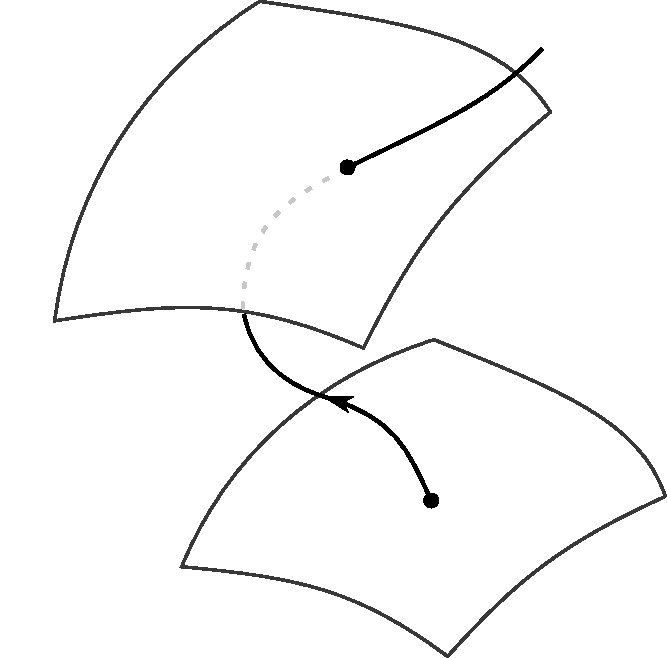
\includegraphics[width=\unitlength]{BeThTrajTeX}}%
    \put(0.28879298,1.02196543){\color[rgb]{0,0,0}\rotatebox{-22.37140782}{\makebox(0,0)[lb]{\smash{$\pS_{\ssp(\zeit)}$}}}}%
    \put(0.55566402,0.45078735){\color[rgb]{0,0,0}\rotatebox{-16.6673442}{\makebox(0,0)[lb]{\smash{$\pS_{\ssp(0)}$}}}}%
    \put(0.63028127,0.18433597){\color[rgb]{0,0,0}\rotatebox{0.03136739}{\makebox(0,0)[lb]{\smash{$\ssp(0)$}}}}%
    \put(0.46253394,0.70182304){\color[rgb]{0,0,0}\rotatebox{0.03136739}{\makebox(0,0)[lb]{\smash{$\ssp(\zeit)$}}}}%
    \put(0.03852492,0.09250899){\color[rgb]{0,0,0}\rotatebox{0.11031334}{\makebox(0,0)[lb]{\smash{$\pS$}}}}%
  \end{picture}%
~~(b)
  \begin{picture}(1,1.07315413)%
    \put(0,0){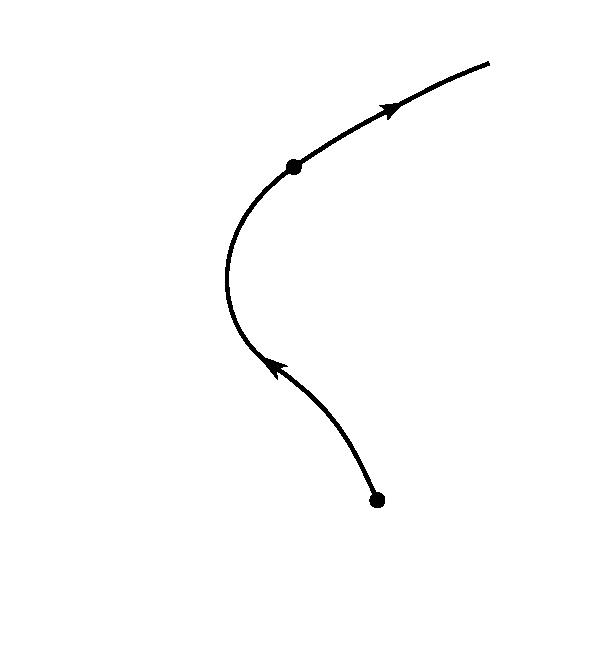
\includegraphics[width=\unitlength]{BeThRedTeX}}%
    \put(0.19912369,0.17144733){\color[rgb]{0,0,0}\rotatebox{0.11031334}{\makebox(0,0)[lb]{\smash{$\pSRed$}}}}%
    \put(0.63028127,0.18433598){\color[rgb]{0,0,0}\rotatebox{0.03136739}{\makebox(0,0)[lb]{\smash{$\sspRed(0)$}}}}%
    \put(0.46253394,0.70182305){\color[rgb]{0,0,0}\rotatebox{0.03136739}{\makebox(0,0)[lb]{\smash{$\sspRed(\zeit)$}}}}%
  \end{picture}%
 \end{center}
% (a) 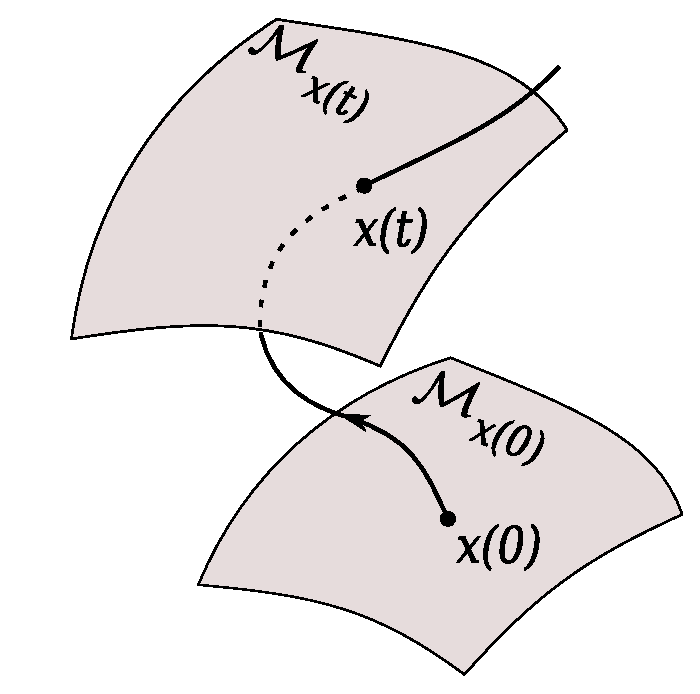
\includegraphics[width=0.45\textwidth]{BeThTraj}
  \caption{\label{fig:BeThTraj}
(a)
The group orbit $\pS_{\ssp(0)}$ of \statesp\ point $\ssp(0)$, and the
group orbit $\pS_{\ssp(\zeit)}$ reached by the trajectory $\ssp(\zeit)$ time $t$
later.
(b)
Symmetry reduction $\pS \to \pSRed$ replaces $\pS_{\ssp}\subset\pS$ by a
single point $\sspRed \in \pSRed$.
  }
\end{figure}
%%%%%%%%%%%%%%%%%%%%%%%%%%%%%%%%%%%%%%%%%%%%%%%%%%

What is a smart way to go about it? Intuition gained from pipe flow (see
\reffig{fig:A27-pipeSymms}), will again prove helpful. A turbulent flow
exhibits a myriad of unstable structures, all traveling down the pipe,
each with its own {\phaseVel}. The
\mslices\rf{rowley_reconstruction_2000,BeTh04,SiCvi10,FrCv11} that we now
describe tells you how to pull each solution back into a {\em fixed}
frame, the \slice, and there compare it to your repertoire of precomputed
solutions, the \template s $\{\slicep{}^{(j)}\}$, by a very geometrical
principle of the closest distance to each. What follows is very much like
the construction of sections of \refsect{s:cut}; due to the linear action
of the symmetry group, slicing is easier than sectioning, but is wholly
unfamiliar - that is why we warmed up by reviewing the \PoincSec s. We
now offer a pictorial tour of this, save for the one bold
incursion\rf{ACHKW11}, hitherto unchartered territory.

First, pick a \template\ $\slicep$ and use the freedom to choose a
moving frame (\reffig{fig:BeThMovFr}\,(b)) to shift and rotate $\slicep$
until it overlies, as well as possible, the state $\ssp$, by minimizing
the distance
\beq
\Norm{\ssp - \LieEl(\gSpace)\,\slicep}
\, .
\ee{minDistance}
The entire group orbit of $\ssp$ is then replaced by the closest match to
the template pattern, given by $\sspRed=\LieEl^{-1}\ssp$. The
symmetry-\reducedsp\ $\pSRed$ is comprised of such closest matches
$\sspRed$, a point for each full \statesp\ group orbit; the hat on
$\sspRed$ indicates the unique point on the group orbit of $\ssp$ closest
to the \template\ \slicep.

%%%%%%%%%%%%%%%%%%%%%%%%%%%%%%%%%%%%%%%%%%%%%%%%%%%%%%%%%%%%%%%%%%%%%
\begin{figure}
	\begin{center}
  	\setlength{\unitlength}{0.25\textwidth}
  	\begin{picture}(1,0.62007592)%
    	\put(0,0){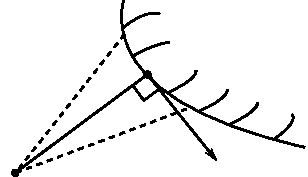
\includegraphics[width=\unitlength]{A28extremum2}}%
    	\put(0.8274739,0.27313042){\color[rgb]{0,0,0}\makebox(0,0)[lb]{\smash{$\LieEl\,\ssp$}}}%
    	\put(0.71822871,0.05712263){\color[rgb]{0,0,0}\makebox(0,0)[lb]{\smash{$\sliceTan{}$}}}%
    	\put(-0.00055527,0.03229441){\color[rgb]{0,0,0}\makebox(0,0)[lb]{\smash{$\slicep$}}}%
    	\put(0.50966967,0.33520145){\color[rgb]{0,0,0}\makebox(0,0)[lb]{\smash{$\sspRed$}}}%
  	\end{picture}
  \end{center}
  \caption{\label{fig:A28extremum}
  Extremal condition \refeq{PCsectQ0} for the point $\sspRed$ on the
  $\ssp$ group orbit that is nearest to the \template\ $\slicep$.
  }
\end{figure}
%%%%%%%%%%%%%%%%%%%%%%%%%%%%%%%%%%%%%%%%%%%%%%%%%%%%%%%%%%%%%%%%%%%%%


The minimal distance satisfies
the extremum condition (\reffig{fig:A28extremum})
\[
\frac{\partial}{\partial \gSpace} \Norm{\ssp - \LieEl(\gSpace)\,\slicep}^2
   =
2\, \braket{\sspRed - \slicep}{\sliceTan{}}
   = 0
        \,,\quad
\sliceTan{} = \Lg \slicep
\,,
\]
where the $[d\!\times\!d]$ matrix $\Lg$ is the generator of infinitesimal
symmetry transformations. $\Norm{\LieEl(\gSpace)\slicep}$ is a constant,
the group tangent vector $\sliceTan{}$ evaluated at $\slicep$
is normal to $\slicep$, and the term
$\braket{\slicep}{\Lg \,\slicep}$ vanishes ($\Lg$ is antisymmetric).
Therefore  $\sspRed$, the point on the group orbit of $\ssp$ that lands
in the \slice, satisfies the \emph{\slice\ condition}
\beq
\braket{\sspRed}{\sliceTan{}} = 0
    \,.
\ee{PCsectQ0}
The \slice\ so defined is thus a $(d\!-\!N)$\dmn\ hyperplane normal to
the $N$ group tangents evaluated at the \slicep. This is sketched in
\reffig{fig:slice}, in a highly idealized manner: A group orbit is a
$N$\dmn\ manifold and even for $\SOn{2}$ it is usually only topologically
a circle, and can intersect a hyperplane any number of times  (see
\reffigs{fig:sliceimage}{fig:chartBord}).

As $\ssp$ varies in time, the {\template} $\slicep$ tracks the motion
using the slice condition \refeq{PCsectQ0} to minimize
$\Norm{\ssp(\zeit)-\LieEl(\phi(\zeit))\slicep}$, and the full-space
trajectory $\ssp(\zeit)$ is thus rotated into the {\reducedsp} $\pSRed$
by appropriate time varying \emph{moving frame} angles
$\{\gSpace(\zeit)\}$, as depicted in \reffig{fig:slice}\,{(a)}. One can
write the equations for the flow in the \reducedsp\, $\dot{\sspRed} =
\velRed(\sspRed)$, which confine the motion to the \slice,
$\sspRed(\zeit) \in \pSRed$, as
\bea
\velRed(\sspRed) &=& \vel(\sspRed)
     \,-\, \dot{\gSpace}(\sspRed) \, \groupTan(\sspRed)
\label{EqMotMFrame}\\
\dot{\gSpace}(\sspRed) &=& \braket{\vel(\sspRed)}{\sliceTan{}}
                       /\braket{\groupTan(\sspRed)}{\sliceTan{}}
\,.
\label{reconstrEq}
\eea
Thus the dynamical system $\{\pS,\map^t\}$ with continuous symmetry
\Group\ is replaced by the {\reducedsp} dynamics $\{\pSRed,\mapRed^t\}$:
with the velocity in the full \statesp\ $\vel$ the sum of $\velRed$, the
velocity component in the \slice, and $\dot{\gSpace}\,\groupTan$, the
velocity component along the group tangent space. The integral of the
{\em reconstruction equation} $\dot{\gSpace}$ keeps track of the group
shift in the full \statesp.

The {\template} $\slicep$ should be a generic \statesp\ point in the
sense that its group orbit has the full $N$ dimensions of the group
\Group. The set of the group orbit points \emph{closest} to the
\template\ \slicep\ forms a neighborhood of \slicep\ in which each group
orbit intersects the hyperplane \emph{only once}. A \slice\ hyperplane
captures neighboring group orbits until, for a point $\sspRSing$ not so
close to the \template, the group tangent vector lies in the \slice. The
group orbits for such points are grazed tangentially rather than sliced
transversally, much like what happens at the \poincBord\
\refeq{eq:sspRSing} for evolution in time. This is also a linear
condition, and it defines the {\sliceBord} ${\cal S}$, a hyperplane in
which both points $\sspRSing$ and their group tangents
$\groupTan(\sspRSing)$ lie in the {\slice},\rf{FrCv11}
\beq
\braket{\sspRSing}{\sliceTan{}} \,=\, 0
      \mbox{ and }
\braket{\groupTan(\sspRSing)}{\sliceTan{}} \,=\, 0
\,.
\label{sliceSingl0}
\eeq
There is yet another, much preferable kind of border: a ridge.
Our initial \slice\ chart $\pSRed{}^{(1)}$ is a ($d\!-\!1$)\dmn\
hyperplane. If we pick another {\template} point $\slicep{}^{(2)}$, it
comes along with its own \slice\ hyperplane $\pSRed{}^{(2)}$. Any pair of
$(d\!-\!1)$\dmn\ local \slice\ hyperplanes intersects in a \emph{ridge},
a $(d\!-\!2)$\dmn\ hyperplane {\PoincS} (drawn in
\reffig{fig:A29-2slices}\,({\it c}) as a `line' and in
\reffig{fig:A29-1ridge} as a `plane' of intersection of two volumes)
shared by a pair of charts and thus satisfies both \slice\ conditions
\refeq{PCsectQ0},
\beq
\braket{\sspRed^*}{\sliceTan{}{}^{(1)}} = 0
\mbox{ and }
\braket{\sspRed^*}{\sliceTan{}{}^{(2)}} = 0
    \,.
\ee{ridge}
We shall refer to the neighborhood of a \template\ \slicep\ bounded by
its {\chartBord} and the ridges to other such linear neighborhoods as a
\emph{chart} $\pSRed_{\slicep} \supset \pS/\Group$, and to
\refeq{sliceSingl0} and \refeq{ridge} as the \emph{border conditions}.
%    \DB{2012-04-13}{\refeq{sliceSingl0} is more restrictive than
%    \refeq{PCsectQ0}. It also defines the slice border rather than a
%    slice.}

%%%%%%%%%%%%%%%%%%%%%%%%%%%%%%%%%%%%%%%%%%%%%%%%%%%%%%%%%%%%%%%%
%% slice.*, inflectHype.*: see dasbuch/book/FigSrc/inkscape/00ReadMe.txt
%% rpo.* hand-drawn in dasbuch/book/FigSrc/xfig/rpo.fig
%% xfig exported -> FigSrc/inkscape/rpo.fig
%% inkscape exported -> rpo.eps + LaTeX, hand edited in the macros
%% Predrag 2011-08-27 replaced rpo.pdf by rpoSlice.pdf
%% remember to insert rpoSlice.pdf into ChaosBook

 \begin{figure}
 \begin{center}
  \setlength{\unitlength}{0.30\textwidth}
  %% \unitlength = units used in the Picture Environment
(a)
  \begin{picture}(1,0.87085079)%
    \put(0,0){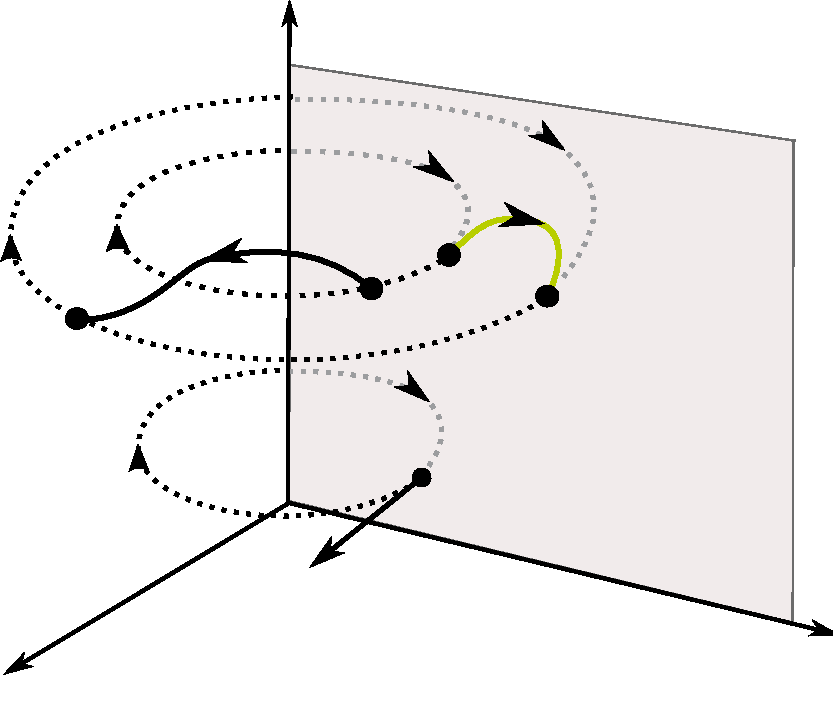
\includegraphics[width=\unitlength]{slice}}%
    \put(0.82835155,0.19007659){\color[rgb]{0,0,0}\rotatebox{-14.84025424}{\makebox(0,0)[lb]{\smash{$\pSRed$}}}}%
    \put(0.06577338,0.28688228){\color[rgb]{0,0,0}\rotatebox{0.0313674}{\makebox(0,0)[lb]{\smash{$\LieEl\,\slicep$}}}}%
    \put(0.53023327,0.26593335){\color[rgb]{0,0,0}\rotatebox{0.0313674}{\makebox(0,0)[lb]{\smash{$\slicep$}}}}%
    \put(0.4284954,0.179285){\color[rgb]{0,0,0}\rotatebox{0.0313674}{\makebox(0,0)[lb]{\smash{$\sliceTan{}$}}}}%
    \put(0.00798985,0.42305068){\color[rgb]{0,0,0}\rotatebox{0.0313674}{\makebox(0,0)[lb]{\smash{$\ssp(\zeit)$}}}}%
    \put(0.65766235,0.45412105){\color[rgb]{0,0,0}\rotatebox{0.0313674}{\makebox(0,0)[lb]{\smash{$\sspRed(\zeit)$}}}}%
    \put(0.06916446,0.74280851){\color[rgb]{0,0,0}\rotatebox{0.0313674}{\makebox(0,0)[lb]{\smash{$\LieEl\,\ssp(\zeit)$}}}}%
  \end{picture}%
\\ %~~~
(b)
  \begin{picture}(1,0.87085079)%
    \put(0,0){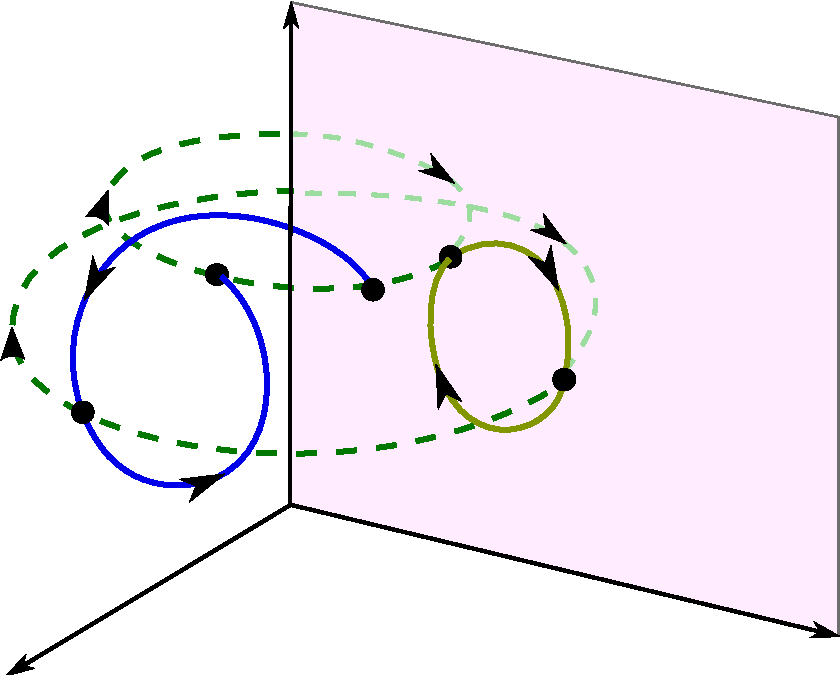
\includegraphics[width=\unitlength]{rpoSlice}}%
    \put(0.82835153,0.19007656){\color[rgb]{0,0,0}\rotatebox{-14.84025432}{\makebox(0,0)[lb]{$\pSRed$}}}%
    \put(0.40925459,0.45713857){\color[rgb]{0,0,0}\rotatebox{0.0313674}{\makebox(0,0)[lb]{\smash{$\ssp(0)$}}}}%
    \put(0.71354118,0.39765314){\color[rgb]{0,0,0}\rotatebox{0.0313674}{\makebox(0,0)[lb]{\smash{$\sspRed(\zeit)$}}}}%
    \put(0.13171187,0.38813817){\color[rgb]{0,0,0}\rotatebox{0.0313674}{\makebox(0,0)[lb]{\smash{$\LieEl(\zeit)$}}}}%
    \put(0.02168739,0.31359574){\color[rgb]{0,0,0}\rotatebox{0.0313674}{\makebox(0,0)[lb]{\smash{$\ssp(\zeit)$}}}}%
    \put(0.15576193,0.48769256){\color[rgb]{0,0,0}\rotatebox{0.0313674}{\makebox(0,0)[lb]{\smash{$\ssp(\period{})$}}}}%
    \put(0.54113911,0.50476963){\color[rgb]{0,0,0}\rotatebox{0.0313674}{\makebox(0,0)[lb]{\smash{$\sspRed(0)$}}}}%
  \end{picture}%
 \end{center}
 \caption{
The \mslices, a \statesp\ visualization:
(a)
\Slice\ $\pSRed \supset \pS/\Group$ lies in the $(d\!-\!N)$\dmn\
hyperplane \refeq{PCsectQ0} normal to $\sliceTan{j}$, which
span the $N$\dmn\ space tangent to the group orbit $\LieEl\,\slicep$
(dotted line) evaluated at the {\template} point $\slicep$. The
hyperplane intersects {all} full \statesp\ group orbits (green
dashes).  The full \statesp\
trajectory $\ssp(\zeit)$ (blue) and the \reducedsp\ trajectory
$\sspRed(\zeit)$ (green) are equivalent up to a `moving frame' rotation
$\ssp(\zeit)=\LieEl(\zeit)\,\sspRed(\zeit)$, where $\LieEl(\zeit)$ is a
shorthand for $\LieEl(\gSpace(\zeit))$.
(b)
In the full \statesp\ a \rpo\ $\ssp(0) \to \ssp(\zeit) \to
\ssp(\period{})$ returns to the group orbit of $\ssp(0)$ after time
$\period{}$ and a rotation by $\LieEl$,  $\ssp(0)=\LieEl \, \ssp
(\period{})$. A generic \rpo\ quasi-\-periodically fills out what is
topologically a torus (\reffig{fig:CLf01group}\,(b)). In the \slice\ $\pSRed$
the symmetry-reduced trajectory is periodic, $\sspRed(0) =
\sspRed(\period{})$.
 }\label{fig:slice}
 \end{figure}



\section{Charting the \slice}
\label{s:chart}

Let us summarize the voyage: We are charting a curved manifold, and it
would be nice to use tools of differential geometry, but try doing it in
61,506\dmn. It will have to be done numerically, and the only feasible
way to do chart this space is to (1) quotient all continuous symmetries,
and (2) tile it with 61,506-$(N+1)$\dmn\ tiles, or `charts'. Here are the
list of tools at hand:

\textbf{\Template.}
Pick a \emph{\template} point $\slicep \in \pS$ such that $\Group$ acts
on it regularly, \ie, whose group orbit is of dimension $N$.

\index{slice}
\textbf{\Slice\ hyperplane.}
We call the $(d\!-\!N)$-dimensional hyperplane
\( %beq
\braket{\sspRed}{\sliceTan{a}}=0
\) %\ee{PCsectQ1}
a \emph{\slice\ hyperplane}.
    \PC{The {\template} should lie outside any of
the invariant subspaces $\pS_H$. Were \slicep\ invariant under the group, then
$\sliceTan{a}=0$ and the `\slice' so defined would be the entire space.
Extend this claim to the invariant subspaces as well}
    \PC{In constructing his return map, Lorenz, I think,
    used projections on the invariant axes $z$ and $\dot{z}$.
    Is that not a \slice? Rethink}
%\end{definition}

\index{moving frame}
\textbf{Moving frame.}
For any $\ssp$, the slice condition  \refeq{PCsectQ0} on $\ssp =
\LieEl(\gSpace)\sspRed$ determines the group action $\LieEl(\gSpace)$ that
brings $ \ssp$ into the \slice.
    \PC{dropped all this: ``The crossing has the same orientation as
    the \template\ group orbit.
    %\beq
    %\braket{\groupTan_{}(\ssp)}{\sliceTan{}} > 0.
    %\ee{SF:orientedSlice}
    In general this will not be sufficient to select unique representative
    and additional constraints are required. If there is a set of angles
    $\{\gSpace_1\leq\gSpace_2\leq\cdots\leq\gSpace_k \}$ that satisfy the
    oriented slice transversal conditions \refeq{PCsectQ0},
    we take the smallest angle $\gSpace_1$.
    problem: this makes sense only for \SOn{2}.
    }
Such a map from a point in the full \statesp\ to the group action
$\gSpace$ is called a \emph{moving
frame}\rf{FelsOlver98,FelsOlver99,OlverInv}.
%\end{definition}

\textbf{\ChartBord.}
The
group orbits for such points are grazed tangentially rather than sliced
transversally, much like what happens at the \poincBord\
\refeq{eq:sspRSing} for evolution in time. This is also a linear
condition, and it defines the {\sliceBord} ${\cal S}$, a hyperplane in
which both points $\sspRSing$ and their group tangents
$\groupTan(\sspRSing)$ lie in the {\slice},\rf{FrCv11}
$
\braket{\sspRSing}{\sliceTan{}} \,=\, 0 $
and
$ \braket{\groupTan(\sspRSing)}{\sliceTan{}} \,=\, 0 \,.$
%\label{sliceSingl0}

\textbf{Ridge.}
There is yet another, much preferable kind of border: a ridge.
Our initial \slice\ chart $\pSRed{}^{(1)}$ is a ($d\!-\!1$)\dmn\
hyperplane. If we pick another {\template} point $\slicep{}^{(2)}$, it
comes along with its own \slice\ hyperplane $\pSRed{}^{(2)}$. Any pair of
$(d\!-\!1)$\dmn\ local \slice\ hyperplanes intersects in a \emph{ridge},
a $(d\!-\!2)$\dmn\ hyperplane {\PoincS}
shared by a pair of charts and thus satisfies both \slice\ conditions,
\(
\braket{\sspRed^*}{\sliceTan{}{}^{(1)}} = 0
\mbox{ and }
\braket{\sspRed^*}{\sliceTan{}{}^{(2)}} = 0
    \,.
\) %ee{ridge}


\textbf{Chart.}
We shall refer to the neighborhood of a \template\ \slicep\ bounded by
its {\chartBord} and the ridges to other such linear neighborhoods as a
\emph{chart} $\pSRed_{\slicep} \supset \pS/\Group$, and to
\refeq{sliceSingl0} and \refeq{ridge} as the {\emph{border conditions}.

Each chart separately describes neighborhood of a single {\template}
point $\slicep$, satisfies the oriented slice transversal condition
\refeq{PCsectQ0}. It is bounded by the \chartBord\ and ridge conditions
\refeq{??}, \refeq{eq:chartBord} that ensure no more than one
group-orbit traversal per chart.

\textbf{Atlas.}
The slice (unique point for each group orbit) is covered by an atlas
consisting of $(d\!-\!1)$\dmn\ charts $\pSRed{}^{(1)}, \pSRed{}^{(2)},
\cdots$

\textbf{\Slice.}
Let $\Group$ act on a $d$-dimensional manifold $\pS$
with its group orbits of dimension $N$ or less. We define a \emph{slice}
to be a $(d\!-\!N)$ dimensional submanifold $\pSRed$ such that all group
orbits that intersect $\pSRed$ do so transversally and only once.
    \PC{dropped `regular', `through a point $\slicep$',
    `in an open neighborhood of $\slicep$'. Does a `manifold' have to be
    smooth, differentiable? Our slice is only continuous}
%\end{definition}

In literature\PC{add refs} `slice' refers to any co-dimension~$N$ surface
that slices transversally, and only once, all group orbits in an open
neighborhood. Here we have defined a
{\slice} constructively but more narrowly, as a contiguous set of
hyperplane charts, with every group orbit accounted for by the atlas
sliced only once, and belonging to a chart.


%%%%%%%%%%%%%%%%%%%%%%%%%%%%%%%%%%%%%%%%%%%%%%%%%%%%%%%%%%%%%%%%%%%%%
\begin{figure}
   \centering
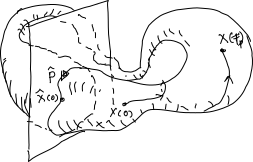
\includegraphics[width=0.40\textwidth]{A29sliceWurst}
   \caption{\label{fig:sliceimage}
Wurst, sliced.
      Every slice hyperplane cuts every group orbit at least twice (see
      \reffig{fig:slice}), once at orbit's closest passage to the
      {\template}, and another time at the most distant passage, also
      satisfying the slice condition \refeq{PCsectQ0}. An $\SOn{2}$ \rpo\
      is topologically a torus, so the two cuts are the two \po\ images
      of the same \rpo, the good close one, and the bad distant one, on
      the other side of {\sliceBord}, and thus not in the slice.
   }
\end{figure}
%%%%%%%%%%%%%%%%%%%%%%%%%%%%%%%%%%%%%%%%%%%%%%%%%%%%%%%%%%%%%%%%%%%%%

%%%%%%%%%%%%%%%%%%%%%%%%%%%%%%%%%%%%%%%%%%%%%%%%%%%%%%%%%%%%%%%%%%%%%%
%\begin{figure}
%   \centering
%  (a)
%~~(b) 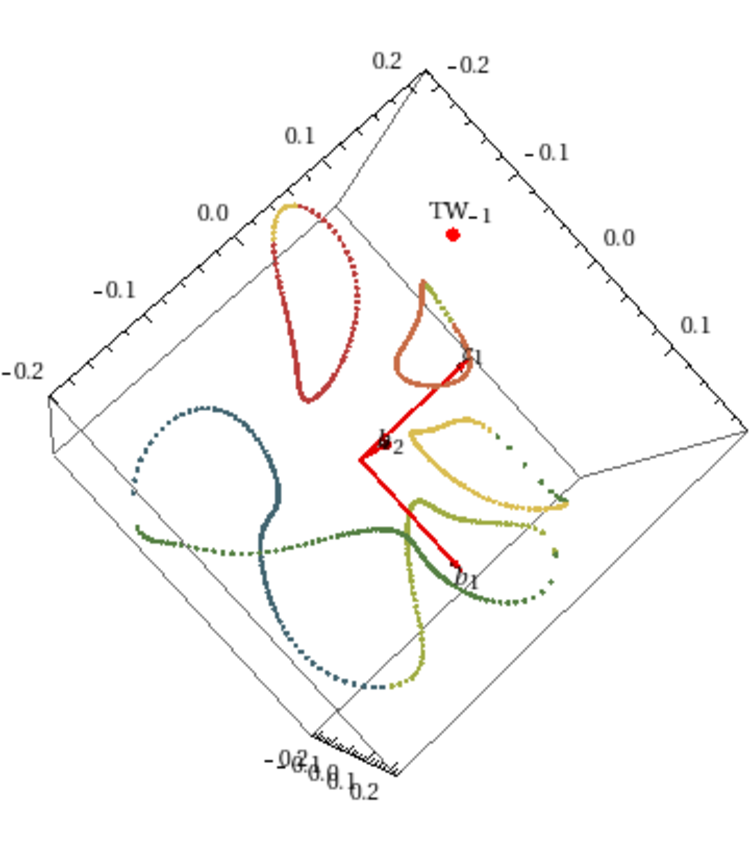
\includegraphics[width=0.45\textwidth]{ks22rpo16mfAll}
%   \caption{ \label{ks22rpo16mf}
%(color online)
%\KS\ \rpo\ with $\period{p}=16.31$, $\shift_p=-2.863$ in a \slice\
%fixed by a \reqv\ \slicep.
%(a)
%(b)
%All intersections of the 2-torus \rpo\ with the \slice\ are plotted.
%Color-coding represents internal numbering of solutions and changes along
%orbits when the number of solutions for $\theta$ changes. We have $3$
%closed-loop images of the \rpo\ and $3$ images that appear to connect to
%a closed loop (from \cite{SiminosThesis}).
%}
%\end{figure}
%%%%%%%%%%%%%%%%%%%%%%%%%%%%%%%%%%%%%%%%%%%%%%%%%%%%%%%%%%%%%%%%%%%%%%

%%%%%%%%%%%%%%%%%%%%%%%%%%%%%%%%%%%%%%%%%%%%%%%%%%%%%%%%%%%%%%%%
 %% chartBord-m*.* replaces FrCv11.tex inflectHype.*
 \begin{figure}
 \begin{center}
  \setlength{\unitlength}{0.30\textwidth}
  %% \unitlength = units used in the Picture Environment
(a)
  \begin{picture}(1,0.91596465)%
    \put(0,0){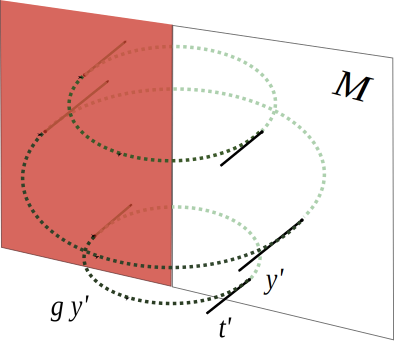
\includegraphics[width=\unitlength]{chartBord-m1}}%
    \put(0.84045332,0.67950567){\color[rgb]{0,0,0}\makebox(0,0)[lb]{\smash{$\pSRed$}}}%
    \put(0.12835189,0.11720037){\color[rgb]{0,0,0}\makebox(0,0)[lb]{\smash{$\LieEl\slicep$}}}%
    \put(0.67299795,0.18547195){\color[rgb]{0,0,0}\makebox(0,0)[lb]{\smash{$\slicep$}}}%
    \put(0.55341875,0.06171734){\color[rgb]{0,0,0}\makebox(0,0)[lb]{\smash{$\sliceTan{}$}}}%
  \end{picture}%
\\
(b)
  \begin{picture}(1,0.91727402)%
    \put(0,0){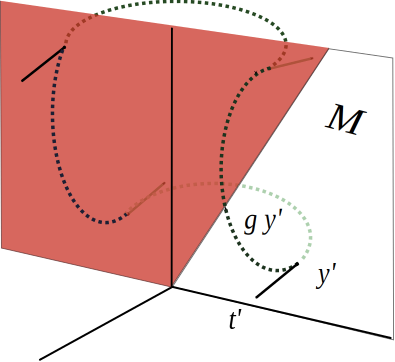
\includegraphics[width=\unitlength]{chartBord-m2}}%
    \put(0.82257887,0.59549577){\color[rgb]{0,0,0}\makebox(0,0)[lb]{\smash{$\pSRed$}}}%
    \put(0.80526889,0.1997715){\color[rgb]{0,0,0}\makebox(0,0)[lb]{\smash{$\slicep$}}}%
    \put(0.57844296,0.0831667){\color[rgb]{0,0,0}\makebox(0,0)[lb]{\smash{$\sliceTan{}$}}}%
    \put(0.61811177,0.33705605){\color[rgb]{0,0,0}\makebox(0,0)[lb]{\smash{$\LieEl\slicep$}}}%
  \end{picture}%
 \end{center}
 \caption{\label{fig:chartBord}  %fig:slice}
\ChartBord: For $\SOn{2}$ two hyperplanes are associated with  a given
{\template} \slicep; the slice $\pSRed$, and the hyperplane of points
$\sspSing$ normal to \refeq{sliceSingl0}, the quadratic Casimir-weighted
vector $\Lg^2\slicep$. The intersection of the two hyperplanes is the
$(d\!-\!2)$\dmn\ hyperplane {\em \chartBord} $\sspRSing \in {\cal S}$, within
which all group tangents $\groupTan(\sspRSing)$ lie in the slice and are
thus normal to $\sliceTan{}$. Beyond this boundary, the group orbits
pierce the \slice\ hyperplane in the wrong direction, so only the
half-hyperplane that contains the \template\ belongs to the slice. The
{\chartBord} is not easy to visualize; For the lack of dimensions, here
it is drawn here as a `line,' the $z$ axis in this 3\dmn\ sketch. (a) If
the equivariant coordinates transform only under the $m=1$ representation
of $\SOn{2}$, every group orbit is a circle, and crosses any
hyperplane twice. However, if there are coordinates that transform as
higher $m$, group orbit can pierce the hyperplane up to $2m$ times, and
the {\chartBord} lies closer to the template. (b) For example, a group
orbit for a combination of $m=1$ and $m=2$ equivariant coordinates
resembles a baseball seam, and can be sliced 4 times, out of which only
the point closest to the \template\ is in the slice (from \wwwcb{}).
 }%
 \end{figure}
%%%%%%%%%%%%%%%%%%%%%%%%%%%%%%%%%%%%%%%%%%%%%%%%%%%%%%%%%%%%%%%%


%%%%%%%%%%%%%%%%%%%%%%%%%%%%%%%%%%%%%%%%%%%%%%%%%%%%%%%%%%%%%%%%
%% A29-2tmplts.* A29-2tmplSl.*
%% Predrag 2012-03-20: see dasbuch/book/FigSrc/inkscape/00ReadMe.txt
%% remember to insert A29-2slices.eps into ChaosBook
 \begin{figure}
 \begin{center}
  \setlength{\unitlength}{0.30\textwidth}
  %% \unitlength = units used in the Picture Environment
(a)\;\;
  \begin{picture}(1,0.92174023)%
    \put(0,0){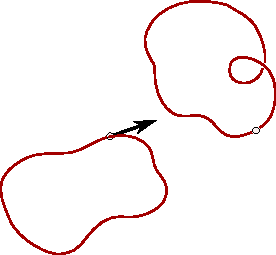
\includegraphics[width=\unitlength]{A29-2tmplts}}%
    \put(0.38186388,0.34995272){\color[rgb]{0,0,0}\makebox(0,0)[lb]{\smash{$\slicep{}^{(1)}$}}}%
    \put(0.41769945,0.50079738){\color[rgb]{0,0,0}\makebox(0,0)[lb]{\smash{$\sliceTan{}{}^{(1)}$}}}%
    \put(0.87339467,0.35886318){\color[rgb]{0,0,0}\makebox(0,0)[lb]{\smash{$\ssp'{}^{(2)}$}}}%
  \end{picture}%
\\
(b)\;\;
  \begin{picture}(1,1.14107266)%
    \put(0,0){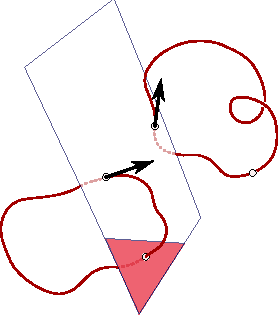
\includegraphics[width=\unitlength]{A29-2tmplSl}}%
    \put(0.54442322,0.48851386){\color[rgb]{0,0,0}\makebox(0,0)[lb]{\smash{$\sliceTan{}{}^{(1)}$}}}%
    \put(0.33649368,0.41474621){\color[rgb]{0,0,0}\makebox(0,0)[lb]{\smash{$\slicep{}^{(1)}$}}}%
    \put(0.41644523,0.62981493){\color[rgb]{0,0,0}\makebox(0,0)[lb]{\smash{$\slicep{}^{(2)}$}}}%
    \put(0.616644,0.84680609){\color[rgb]{0,0,0}\makebox(0,0)[lb]{\smash{$\sliceTan{}{}^{(2)}$}}}%
    \put(0.88017597,0.4261647){\color[rgb]{0,0,0}\makebox(0,0)[lb]{\smash{$\ssp'{}^{(2)}$}}}%
    \put(0.29194797,0.95658666){\color[rgb]{0,0,0}\makebox(0,0)[lb]{\smash{$\pSRed{}^{(1)}$}}}%
  \end{picture}%
 \end{center}
 \caption{\label{fig:A29-2tmplts}
A 2-chart atlas. Sketch
    (a)
depicts two templates $\slicep{}^{(1)}$, $\ssp'{}^{(2)}$, each with its
group orbit. Start with the {\template} $\slicep{}^{(1)}$. All group
orbits traverse its $(d\!-\!1)$\dmn\ slice hyperplane, including the
group orbit of the second {\template} $\ssp'{}^{(2)}$.
    (b)
Replace the second
{\template} by its closest group-orbit point $\slicep{}^{(2)}$, \ie, the
point in \slice\ $\pSRed{}^{(1)}$. This is allowed as long as  $\slicep{}^{(2)}$ is
closer than the $\pSRed{}^{(1)}$ {\chartBord} (red region), otherwise an interpolating,
closer template needs to be introduced.
(from \wwwcb{}).
 }
 \end{figure}
%%%%%%%%%%%%%%%%%%%%%%%%%%%%%%%%%%%%%%%%%%%%%%%%%%%%%%%%%%%%%%%%


%%%%%%%%%%%%%%%%%%%%%%%%%%%%%%%%%%%%%%%%%%%%%%%%%%%%%%%%%%%%%%%%
%% A29-2slices.* A29-2charts.*
%% Predrag 2012-03-20: see dasbuch/book/FigSrc/inkscape/00ReadMe.txt
%% remember to insert A29-2slices.eps into ChaosBook
 \begin{figure}
 \begin{center}
  \setlength{\unitlength}{0.40\textwidth}
  %% \unitlength = units used in the Picture Environment
(c)\;\;
  \begin{picture}(1,0.86567815)%
    \put(0,0){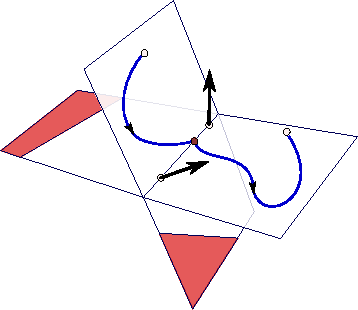
\includegraphics[width=\unitlength]{A29-2slices}}%
    \put(0.3850416,0.38725438){\color[rgb]{0,0,0}\makebox(0,0)[lb]{\smash{$\slicep{}^{(1)}$}}}%
    \put(0.60194012,0.48012421){\color[rgb]{0,0,0}\makebox(0,0)[lb]{\smash{$\slicep{}^{(2)}$}}}%
    \put(0.4042968,0.74412842){\color[rgb]{0,0,0}\makebox(0,0)[lb]{\smash{$\sspRed(0)$}}}%
    \put(0.79647438,0.54627847){\color[rgb]{0,0,0}\makebox(0,0)[lb]{\smash{$\sspRed(\zeit)$}}}%
  \end{picture}%
\\
(d)\;\;
  \begin{picture}(1,0.5127804)%
    \put(0,0){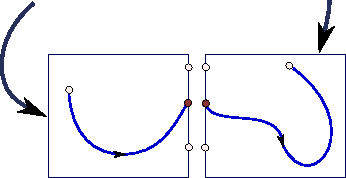
\includegraphics[width=\unitlength]{A29-2charts}}%
    \put(0.16199231,0.03841546){\color[rgb]{0,0,0}\makebox(0,0)[lb]{\smash{$\pSRed{}^{(1)}$}}}%
    \put(0.63051777,0.0374085){\color[rgb]{0,0,0}\makebox(0,0)[lb]{\smash{$\pSRed{}^{(2)}$}}}%
    \put(0.21517269,0.28787637){\color[rgb]{0,0,0}\makebox(0,0)[lb]{\smash{$\sspRed(0)$}}}%
    \put(0.75921701,0.25014044){\color[rgb]{0,0,0}\makebox(0,0)[lb]{\smash{$\sspRed(\zeit)$}}}%
    \put(0.60952792,0.26511997){\color[rgb]{0,0,0}\makebox(0,0)[lb]{\smash{$\slicep{}^{(2)}$}}}%
    \put(0.45827029,0.02997228){\color[rgb]{0,0,0}\makebox(0,0)[lb]{\smash{$\slicep{}^{(1)}$}}}%
  \end{picture}%
 \end{center}
 \caption{\label{fig:A29-2slices}
A 2-chart atlas.
    (c)
Now that the group orbits have been reduced to points, erase them and
consider the two slices through the two {\template s}. As these two
{\template s} are the closest points viewed from either group orbit, they
lie in both \slice s. However, the two tangent vectors
$\sliceTan{}{}^{(1)}$ and $\sliceTan{}{}^{(2)}$ have different
orientations, so they define two distinct \slice\ hyperplanes
$\pSRed{}^{(1)}$ and $\pSRed{}^{(2)}$ which intersect in the
\emph{ridge}, a hyperplane of dimension $(d\!-\!2)$ (here drawn as a
`line,' and in \reffig{fig:A29-1ridge} as intersection of two `volumes')
shared by the template pair that satisfies both \slice\ conditions
\refeq{ridge}. The chart for the neighborhood of each template (a page of
the atlas in part (d)) extends only as far as this ridge. If the
templates are sufficiently close, the {\chartBord} of each \slice\ (red
region) is beyond this ridge, and not encountered by the symmetry-reduced
trajectory $\sspRed(\zeit)$. The reduced trajectory is continuous in the
slice comprised of such charts - it switches the chart whenever it
crosses a ridge.
    (d)
The slice (unique point for each group orbit) is now covered by an atlas
consisting of $(d\!-\!1)$\dmn\ charts $\pSRed{}^{(1)}, \pSRed{}^{(2)},
\cdots$
(from \wwwcb{}).
 }
 \end{figure}
%%%%%%%%%%%%%%%%%%%%%%%%%%%%%%%%%%%%%%%%%%%%%%%%%%%%%%%%%%%%%%%%

%%%%%%%%%%%%%%%%%%%%%%%%%%%%%%%%%%%%%%%%%%%%%%%%%%%%%%%%%%%%%%%%
%% A29-1ridge.*
%% Predrag 2012-03-30: see dasbuch/book/FigSrc/inkscape/00ReadMe.txt
%% remember to insert A29-1ridge.eps into ChaosBook
 \begin{figure}
 \begin{center}
  \setlength{\unitlength}{0.40\textwidth}
  %% \unitlength = units used in the Picture Environment
  \begin{picture}(1,0.89907101)%
    \put(0,0){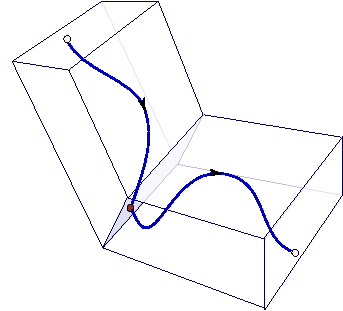
\includegraphics[width=\unitlength]{A29-1ridge}}%
    \put(0.00894598,0.81885604){\color[rgb]{0,0,0}\makebox(0,0)[lb]{\smash{$\sspRed(0)$}}}%
    \put(0.88743345,0.05105926){\color[rgb]{0,0,0}\makebox(0,0)[lb]{\smash{$\sspRed(\zeit)$}}}%
    \put(0.78614059,0.43443027){\color[rgb]{0,0,0}\rotatebox{-25.76142111}{\makebox(0,0)[lb]{\smash{$\pSRed{}^{(2)}$}}}}%
    \put(0.37048948,0.79485578){\color[rgb]{0,0,0}\rotatebox{-61.41291822}{\makebox(0,0)[lb]{\smash{$\pSRed{}^{(1)}$}}}}%
    \put(0.2429401,0.27697318){\color[rgb]{0,0,0}\makebox(0,0)[lb]{\smash{$\sspRed_2$}}}%
    \put(0.47832196,0.33514069){\color[rgb]{0,0,0}\makebox(0,0)[lb]{\smash{$\sspRed_1$}}}%
  \end{picture}%
 \end{center}
 \caption{\label{fig:A29-1ridge}
Here the two charts of \reffig{fig:A29-2slices}\,({\it c}) are drawn as two
$(d\!-\!1)$\dmn\ slabs. Ridge, their $(d\!-\!2)$\dmn\ intersection can then be
drawn as the shaded plane. This hyperplane
cuts across the symmetry-reduced trajectory $\sspRed(\zeit)$ and thus
serves as a \PoincSec\ that captures all oriented transits from
the neighborhood of {\template} $\slicep{}^{(1)}$ to the
neighborhood of {\template} $\slicep{}^{(2)}$. \PoincSec\ transits
are oriented, so $\sspRed_1$ and $\sspRed_2$ are in the section, but
the third point is not.
(from \wwwcb{}).
 }
 \end{figure}
%%%%%%%%%%%%%%%%%%%%%%%%%%%%%%%%%%%%%%%%%%%%%%%%%%%%%%%%%%%%%%%%

A local hyperplane segment of the \slice\ is good only up to the
\sliceBord\ and or the ridge.


The rest is geometry of hyperplanes, nothing to do with dynamics, only
with the group theory. In particular, while we motivated slicing by
emphasizing that the choice of templates is where the nonlinear physics
enters, the \slice, \chartBord\ and ridge conditions \refeq{PCsectQ0},
\refeq{eq:chartBord} and \refeq{ridge} are all linear conditions which
depend on the ray defined by the \template\ \slicep, not its magnitude.
Checking whether the {\chartBord} is on the far side of the ridge between
two \slice s is a linear computation; for a symmetry-reduced trajectory
moving in $\pSRed{}^{(1)}$ slice one only has to keep checking the sign
of
\beq
\braket{\sspRed(\zeit)}{\sliceTan{}{}^{(2)}}
\,.
\ee{eq:chartBord}
Once this changes the sign, the ridge has been crossed, and from then on
the trajectory should be reduced to the $\pSRed{}^{(2)}$ slice.

Group orbits $\pS_{\slicep}$, group tangents $\groupTan(\slicep)$ and the
associated \slice s are purely group-theoretic, linear concepts: they
know nothing about dynamics. Dynamics enters only through informed
choices of \template s.

The physical task is to, for a given dynamical flow, pick a set of
qualitatively distinct {\template s} (for example, for a turbulent pipe
flow, one typical of 2-roll states, one for 4-roll states, and so on)
whose \slice s  are locally transverse to open sets of nearby orbits, and
which together provide a good atlas for the region of $\pS/\Group$
explored by chaotic trajectories. Each chart $\pS{}^{(j)}$ covers a
neighborhood of an important, qualitatively distinct class of solutions,
of features qualitatively captured by \template\ $\slicep{}^{(j)}$.
Together they provide an atlas -a finite set of hyperplane tiles-
charting the regions of the curved manifold explored by the trajectories
of interest.

%%%%%%%%%%%%%%%%%%%%%%%%%%%%%%%%%%%%%%%%%%%%%%%%%
% 2011-09-09, 2012-03-30 Predrag: add BeThMovFr to
%            continuous.tex overheads, and ChaosBook
% replace A27movFrame*.* everywhere
\begin{figure}
 \begin{center}
(a) 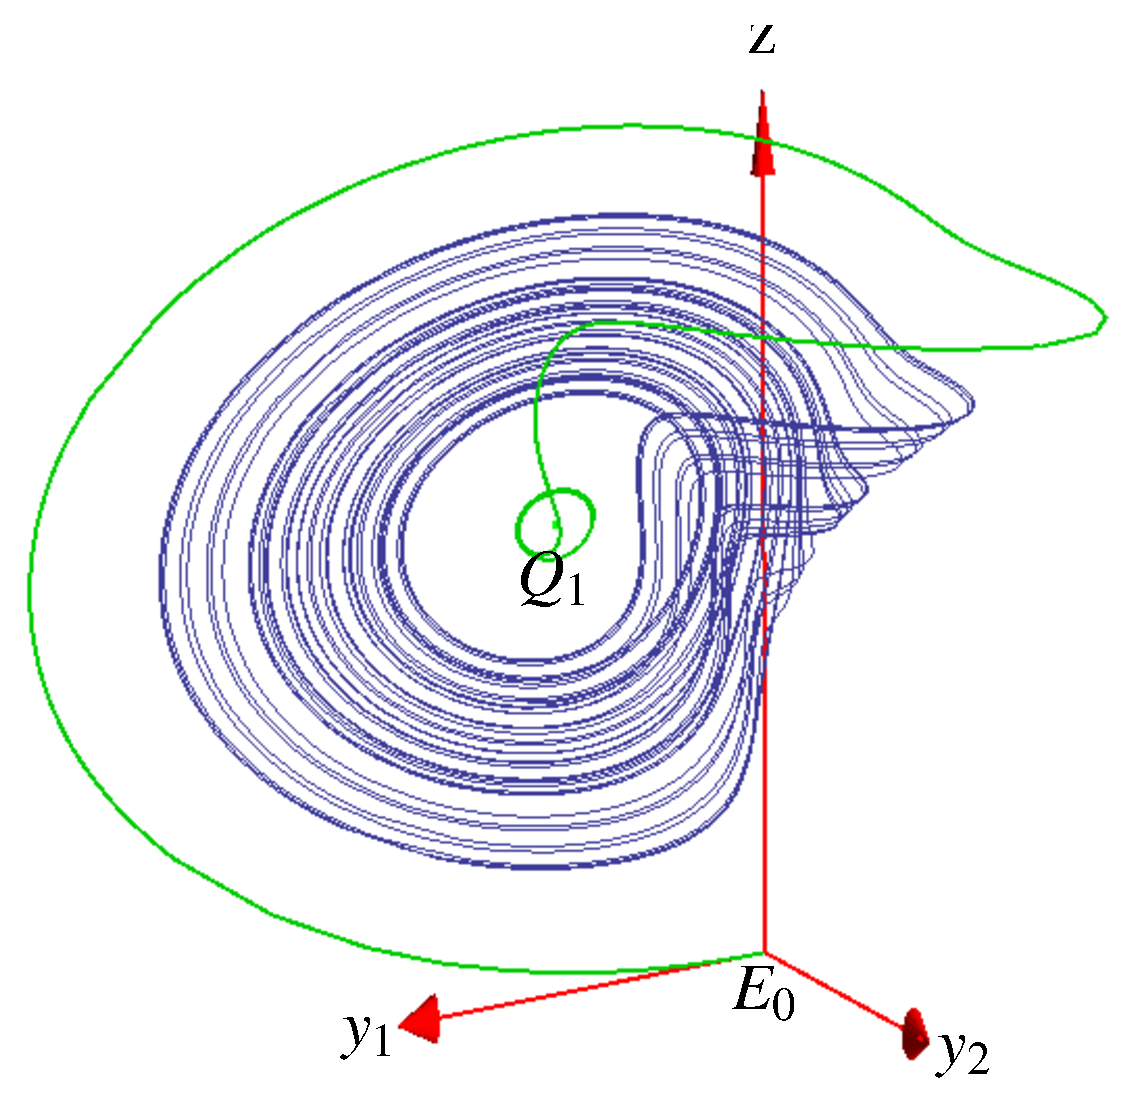
\includegraphics[width=0.20\textwidth]{CLEperpReqb}
(b) 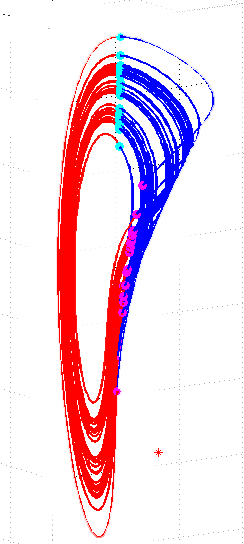
\includegraphics[width=0.16\textwidth]{cLe-2chartsDB}
 \end{center}
  \caption{\label{fig:cLe-2charts}
(a)
\mycomment{\DBedit{\Huge [DRAW THIS!]}}{}
Strange attractor of the \cLe\ in a single \slice, \template\
the \reqv\ $\slicep = \ssp_{\REQV{}{1}}$ exhibits singular jumps
(from \refref{SiCvi10}).
(b)
\mycomment{\DBedit{\Huge [DRAW THIS!]}}{}
The 2-chart atlas (sketched in \reffig{fig:A29-1ridge}) of the strange
attractor of the \cLe, with the ridge \PoincSec\ points
$\sspRed^* \in \PoincS$ marked green (and the wrong direction section
crossings marked purple).
  }
\end{figure}
%%%%%%%%%%%%%%%%%%%%%%%%%%%%%%%%%%%%%%%%%%%%%%%%%%


    \ifdraft\color{blue}
{\bf What it is not}
    \begin{itemize}
      \item reduced-dimensionality model: Symmetry reduction is not a
          dimensional-reduction scheme, or flow modeling by fewer degrees
          of freedom: it is a local change of coordinate, with one (or
          $N$) coordinates pointing along the phase directions. The
          $(d\!-\!N)$\dmn\ \reducedsp\ is also $\infty$-dimensional and
          no information is lost, one can go freely between solutions in
          the full and reduced \statesp s by integrating the associated
          {reconstruction equations} \refeq{reconstrEq}.
      \item an atlas is \emph{not needed} for Newton determination of a
            single trajectory; any local section and slice plus time and shift
            constraints is OK, can even move them with each Newton
            iteration. 60,000 \rpo s can be computed\rf{SCD07} this way.
            The question is: what then? and for that you need a good atlas.
    \end{itemize}



\section{Bridges to nowhere}
\label{s:bridge}

You can safely skip this section, unless you would like to join a brief
tour of the graveyard of obvious ideas and pet symmetry reduction schemes
that all have one thing in common: they do not work.

Everybody and her mother encounters a symmetry sooner or later, so
literature on symmetry reduction is vast.
For a history, see remarks in ChaosBook.org and \refref{SiCvi10}.


{\bf Method of connections}

example: swimmer

%%%%%%%%%%%%%%%%%%%%%%%%%%%%%%%%%%%%%%%%%%%%%%%%%%%%%%%%%%%%%%%%%%%%%
\begin{figure}
   \centering
  \setlength{\unitlength}{0.20\textwidth}
(a)~~~
  \begin{picture}(1,0.98073806)%
    \put(0,0){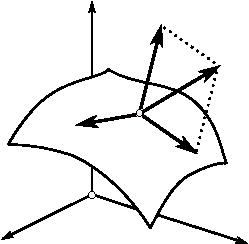
\includegraphics[width=\unitlength]{A28tangents}}%
    \put(0.8635648,0.73622308){\color[rgb]{0,0,0}\makebox(0,0)[lb]{\smash{$\vel$}}}%
    \put(0.49893205,0.86039365){\color[rgb]{0,0,0}\makebox(0,0)[lb]{\smash{$\vel_{\bot}$}}}%
    \put(0.27198728,0.5378933){\color[rgb]{0,0,0}\makebox(0,0)[lb]{\smash{$\groupTan_1$}}}%
    \put(0.58493215,0.33483773){\color[rgb]{0,0,0}\makebox(0,0)[lb]{\smash{$\groupTan_2$}}}%
    \put(0.54959234,0.21257862){\color[rgb]{0,0,0}\makebox(0,0)[lb]{\smash{$\LieEl\ssp$}}}%
  \end{picture}%
(b)~~~
  \begin{picture}(1,0.98655417)%
    \put(0,0){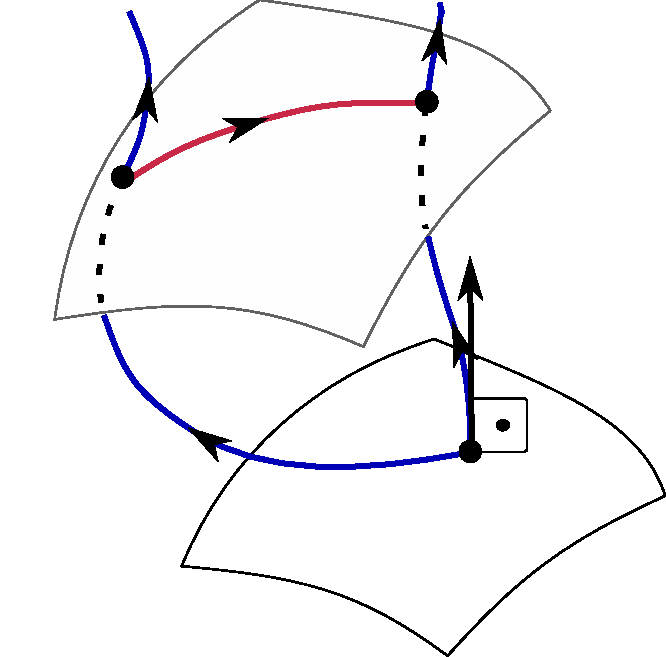
\includegraphics[width=\unitlength]{BeThMconnect}}%
    \put(0.20559239,0.64023845){\color[rgb]{0,0,0}\rotatebox{0.0313674}{\makebox(0,0)[lb]{\smash{$\ssp(\zeit)$}}}}%
    \put(0.68383186,0.20519203){\color[rgb]{0,0,0}\rotatebox{0.0313674}{\makebox(0,0)[lb]{\smash{$\ssp(0)$}}}}%
    \put(0.67475925,0.8109461){\color[rgb]{0,0,0}\rotatebox{0.0313674}{\makebox(0,0)[lb]{\smash{$\sspRed(\zeit)$}}}}%
    \put(0.35760559,0.8662057){\color[rgb]{0,0,0}\rotatebox{0.0313674}{\makebox(0,0)[lb]{\smash{$\LieEl(\zeit)$}}}}%
    \put(0.70884327,0.61850672){\color[rgb]{0,0,0}\rotatebox{0.0313674}{\makebox(0,0)[lb]{\smash{$\vel_{\bot}$}}}}%
  \end{picture}%
   \caption{\label{fig:BeThMconnect}
    (a)
By equivariance $\vel(\ssp)$ can be replaced by $\vel_\bot(\ssp)$, the
velocity normal to the group tangent directions at \statesp\ point $\ssp$.
    (b)
Method of connections replaces $\vel(\sspRed)$ at every instant
$\sspRed =\sspRed(\zeit)$ by $\vel_\bot(\sspRed)$, so in
$\sspRed(\zeit)$ co-moving frame there is no motion along the group
tangent directions.
}
\end{figure}
%%%%%%%%%%%%%%%%%%%%%%%%%%%%%%%%%%%%%%%%%%%%%%%%%%%%%%%%%%%%%%%%%%%%%

    \ifdraft\color{blue}
still to discuss:
    \begin{itemize}
      \item refer to \reffig{fig:BeThMconnect}
      \item cite Shapere and Wilczek Geometric Phase collection

      \item gauge fixing = moving frames

      \item geometric phase?

  \item strobing $\sim$ method of connections

  \item reduction vs projection
    \end{itemize}
    \color{black}\fi


{\bf A co-moving frame}
Visualizing a single `relative' trajectory in its co-moving frame, moving with
the mean {\phaseVel} of a given solution, is useful if we are
concerned with that individual solution.
    \PC{cite Golubitsky}
A co-moving frame is useless if
we are concerned with studying collections of these trajectories, as each
solution travels with its own mean {\phaseVel}, and there is no single
co-moving frame that can simultaneously reduce \emph{all} traveling
solutions.

disparage co-moving frames: they are misleading for \rpo s, as they
    misrepresent time segments for which a \po\ might be glued to
    barely unstable \eqv. A co-moving frame rotates with the constant
    mean
    $\timeAver{\velRel}= \shift_p/\period{p}
    \,.
    $ We \emph{emphatically} do not work in
    co-moving frames.

unhappy about ``moving frames'': misleading, as slice is
     \emph{emphatically} stationary. ''Covariant frames'' move, but we
     do not know how to use them

    %\PC{2012-04-12 - reuse this?: ``
    As long as one is focusing on a single solution of \NSe, there are many
    excellent, physically insightful $3D$ visualizations of the flow:
    velocity fields on flow sections, isovorticity surfaces, videos of the
    flow, and so on. But today we own dozens of exact \eqv\ and \reqv\
    solutions for a given turbulent flow, and we are commencing an exploration of
    states of turbulent fluids in terms of the unstable \po\ solutions whose
    number, as a function of the increasing period, is growing exponentially.
    How are we to visualize \emph{the totality} of these solutions in one go?


Purely group-theoretical, no dynamics to inform it.

{\bf Polar coordinates}

even for pipe flows one does not use cylindrical Bessel functions
eigenbasis.

{\bf Hilbert bases}

%    \DB{2012-04-10}
%    {A book report on Hilbert bases by Daniel Borrero}
One approach to symmetry reduction that is often used for low-dimensional
dynamical systems is to rewrite the dynamics in terms of a Hilbert
invariant polynomial basis (see \refref{GL-Gil07b} for a clear and
detailed discussion of this method). The idea here is that one can take
the dynamics in equivariant state space coordinates
$(x_1,x_2,x_3,...,x_d)$ and rewrite them in terms of polynomials of these
variables $(u_1,u_2,u_3,...,u_m)$ that are invariant under the group
action. The algebra required is quite involved and the required
computations become very large for problems with as few as ten
dimensions\rf{gatermannHab}. This makes the method of Hilbert bases
unfeasible for dealing with high-dimensional dynamical systems, such
as turbulent fluid flows.

{\bf Marsdenmania}

Hamiltonian, more complicated

    \color{black}\fi


\section{Conclusions}
\label{s:concl}

As a turbulent flow evolves, every so often we catch a glimpse of a
familiar structure. For any finite spatial resolution, the flow follows
for a finite time an unstable {\cohStr} belonging to an alphabet of
representative states, here called `\template s'. In presence of
symmetries, near recurrences can be identified only if shifted both in
time and space.

In the method of sections (along time direction) and slices (along
spatial symmetry directions) the identification of physically close
states is achieved by cutting the group orbits with a finite set of
hyperplanes, one for each continuous parameter, with each time trajectory
and group orbit of symmetry-equivalent points represented by a single
point, its  section and \slice.
The \mslices\ is akin to (but distinct from) cutting across trajectories
by means of sections. Both methods reduce continuous symmetries: one
sections the continuous-time trajectories, the other slices the layers of
the onion formed by group-orbits. Both are triggered by kin
conditions: oriented piercing of the section, oriented piercing of the slice. Just
as a \PoincSec\ goes bad, the slice goes bad the moment transversality is
lost. \Slice, however, is emphatically \emph{not} a \PoincSec; it
replaces a trajectory by a symmetry-reduced trajectory, whereas a
\PoincSec\ replaces a continuous time trajectory by a sequence of points.

%    \PC{2011-10-18 incorporate this paragraph:
Note also that symmetry reduction is not a dimensional-reduction scheme,
or flow modeling by fewer degrees of freedom: the \reducedsp\ retains the
full dimensionality of the original dynamical systems. No information is
lost, one can go freely between solutions in the full and reduced
\statesp s by integrating the associated {reconstruction equations}.

The main message of this visual tour is that if a dynamical problem has a
continuous symmetry, the symmetry \emph{must} be reduced before any
detailed analysis of flow's \statesp\ geometry can commence. So far, this
has only been achieved for transitionally turbulent numerical pipe
flows\rf{ACHKW11}, resulting in the discovery of the first \rpo s
embedded in turbulence. In future it should be the first step in analysis
of any turbulent data, numerical\rf{CvGr12} or experimental\rf{BCS12}.
Once symmetry reduction is achieved, all solutions of a turbulent
flow can be plotted together, as one happy family: all
symmetry-equivalent states are represented by a single point, families of
solutions are mapped to a single solution, \reqva\ become \eqva, \rpo s
become \po s, and the global dynamical systems analysis if terms of
invariant solutions and their stable / unstable manifolds can now commence.

\begin{acknowledgments}
This article answers the questions asked after the talk given at
Kyoto 2011 IUTAM Symposium on ``50 Years of Chaos: Applied and Theoretical.''
We are indebted to
S.~Froehlich,
E.~Siminos,
S.A.~Solla,
and
R.~Wilczak
for inspiring discussions.
P.~C.\ thanks G.~Robinson,~Jr.\ for support,
Max-Planck-Institut f\"ur Dynamik und Selbstorganisation,
G\"ottingen for hospitality,
and the Nieders\"achsischen Knackwurst and Bayerische Hefeweizen for inspiration.
P.~C.\ was partly supported by NSF grant DMS-0807574
and
2009 Forschungspreis der Alexander von Humboldt-Stiftung.
\end{acknowledgments}


% \bibliographystyle{jfm}
% \nocite{*}
\bibliography{../bibtex/siminos}

\ifdraft
    \onecolumngrid

    \newpage
\input figures
    \newpage
\input flotsam
    \newpage
    \section{Daily blog, point by point}
    \label{chap:atlas}
\input ../blog/atlas
\fi

\end{document}
